% lecture7.tex -- GENERATED by build_L7.py from L7_numbers.json; do not edit by hand.
\documentclass[10pt,aspectratio=169,t]{beamer}
% =============================================================================
% nn_preamble.tex -- shared Beamer preamble of Neural Networks and Deep Learning (NN)
% Used by every lecture: lectures/Lk/lecturek.tex does
%   \documentclass[10pt,aspectratio=169,t]{beamer}
%   % =============================================================================
% nn_preamble.tex -- shared Beamer preamble of Neural Networks and Deep Learning (NN)
% Used by every lecture: lectures/Lk/lecturek.tex does
%   \documentclass[10pt,aspectratio=169,t]{beamer}
%   % =============================================================================
% nn_preamble.tex -- shared Beamer preamble of Neural Networks and Deep Learning (NN)
% Used by every lecture: lectures/Lk/lecturek.tex does
%   \documentclass[10pt,aspectratio=169,t]{beamer}
%   \input{../common/nn_preamble}
%   \nnlecture{k}{Lecture title}
% Logos live in lectures/common/logos/, charts in lectures/Lk/charts/.
% Do NOT add \hfuzz / \vfuzz / \hbadness here: overfull boxes must be fixed, not hidden.
% =============================================================================

\usetheme{default}
\setbeamersize{text margin left=7mm, text margin right=7mm}

% ---------------------------------------------------------------- packages
\usepackage[utf8]{inputenc}
\usepackage[T1]{fontenc}
\usepackage{lmodern}
\usepackage{amsmath, amssymb}
\usepackage{mathtools}
\usepackage{bm}
\usepackage{tikz}
\usetikzlibrary{arrows.meta, positioning, calc, shapes.misc}
\usepackage{booktabs}
\usepackage{array}
\usepackage{graphicx}
\usepackage{colortbl}
\usepackage{xcolor}
\usepackage{multicol}
\hypersetup{colorlinks=true, linkcolor=MainBlue, urlcolor=MainBlue, citecolor=MainBlue}
\graphicspath{{../common/logos/}}   % charts are included with their language folder: charts/en/, charts/ro/

% ---------------------------------------------------------------- colours
\definecolor{MainBlue}{RGB}{26, 58, 110}
\definecolor{IDAred}{RGB}{205, 0, 0}
\definecolor{DarkGray}{RGB}{51, 51, 51}
\definecolor{FooterGray}{RGB}{100, 100, 100}
\definecolor{BlockGray}{RGB}{236, 238, 242}
\definecolor{KeynoteGray}{RGB}{218, 218, 218}
\definecolor{Crimson}{RGB}{190, 40, 50}
\definecolor{Forest}{RGB}{30, 110, 50}
\definecolor{Bitter}{RGB}{214, 150, 20}
% chart palette (same hex values and order as lectures/common/nn_plot.py SERIES)
\definecolor{Ser1}{HTML}{2A78D6}
\definecolor{Ser2}{HTML}{EB6834}
\definecolor{Ser3}{HTML}{1BAF7A}
\definecolor{Ser4}{HTML}{EDA100}
\definecolor{Ser5}{HTML}{E87BA4}
\definecolor{Ser6}{HTML}{008300}
\definecolor{Ser7}{HTML}{6250D6}
\definecolor{Ser8}{HTML}{E34948}

\setbeamertemplate{background}{%
  \begin{tikzpicture}[remember picture, overlay]
    \shade[shading=axis, shading angle=315, top color=white, bottom color=KeynoteGray]
      (current page.south west) rectangle (current page.north east);
  \end{tikzpicture}}
\setbeamercolor{background canvas}{bg=}
\setbeamercolor{structure}{fg=MainBlue}
\setbeamercolor{normal text}{fg=DarkGray}
\setbeamercolor{title}{fg=IDAred}
\setbeamercolor{frametitle}{fg=IDAred, bg=}
\setbeamercolor{block title}{bg=MainBlue, fg=white}
\setbeamercolor{block body}{bg=BlockGray, fg=DarkGray}
\setbeamercolor{block title alerted}{bg=Crimson, fg=white}
\setbeamercolor{block body alerted}{bg=Crimson!7, fg=DarkGray}
\setbeamercolor{block title example}{bg=Forest, fg=white}
\setbeamercolor{block body example}{bg=Forest!7, fg=DarkGray}
\setbeamercolor{item}{fg=MainBlue}
\setbeamerfont{frametitle}{size=\large, series=\bfseries}
\setbeamerfont{block title}{size=\small, series=\bfseries}
\setbeamertemplate{blocks}[rounded][shadow=false]
\setbeamertemplate{itemize item}{\color{MainBlue}$\boxdot$}
\setbeamertemplate{itemize subitem}{\color{MainBlue}\scriptsize$\blacktriangleright$}
% compact two-level lists: level 1 = main point, level 2 = details (no text outside bullets)
\setbeamerfont{itemize/enumerate subbody}{size=\footnotesize}
\setlength{\leftmargini}{1.1em}
\setlength{\leftmarginii}{1.1em}
\setbeamertemplate{itemize/enumerate body begin}{\setlength{\topsep}{0pt}\setlength{\partopsep}{0pt}\setlength{\parskip}{0pt}}
\setbeamertemplate{itemize/enumerate subbody begin}{\setlength{\topsep}{0pt}\setlength{\partopsep}{0pt}\setlength{\itemsep}{0pt}\vspace{-0.4ex}}

\setbeamertemplate{enumerate item}{\color{MainBlue}\insertenumlabel.}
\setlength{\leftmargini}{1.3em}
\setlength{\leftmarginii}{1.2em}
\setbeamertemplate{navigation symbols}{}
\setbeamertemplate{section in toc}{\color{MainBlue}$\blacktriangleright$~\inserttocsection}
\setbeamertemplate{caption}{\raggedright\insertcaption\par}
% frame subtitle = precise citation line under the claim title (Weron style)
\setbeamerfont{framesubtitle}{size=\footnotesize}
\setbeamercolor{framesubtitle}{fg=FooterGray}
% outline that reappears at every section with the current section highlighted
\setbeamertemplate{section in toc shaded}[default][35]
\setbeamertemplate{subsection in toc shaded}[default][35]
\setbeamertemplate{subsection in toc}{\leavevmode\leftskip=2.2em\color{DarkGray}\small\inserttocsubsection\par}
\AtBeginSection[]{{\begin{frame}{\txtoutline}\vspace{2mm}\small
  \tableofcontents[currentsection,hideothersubsections]\end{frame}}}

% ---------------------------------------------------------------- head and foot
\setbeamertemplate{headline}{%
  \vskip10pt%
  \hbox to \paperwidth{\hskip0.5cm%
    {\small\color{FooterGray}\renewcommand{\hyperlink}[2]{##2}\insertsectionhead}%
    \hfill\textcolor{FooterGray}{\small\insertframenumber}\hskip0.5cm}%
  \vskip4pt{\color{FooterGray}\hrule height 0.4pt}}
% footer as in the other courses (MFM, SFM): course name on the left, small sparkline on the right
\setbeamertemplate{footline}{%
  {\color{FooterGray}\hrule height 0.4pt}\vskip4pt%
  \hbox to \paperwidth{\hskip0.5cm%
    \textcolor{FooterGray}{\small\txtcourse}%
    \hfill\raisebox{-0.1em}{\begin{tikzpicture}[x=0.08em, y=0.08em, line width=0.4pt]
      \draw[FooterGray] (0,3) -- (1,4) -- (2,3.5) -- (3,5) -- (4,4) -- (5,6) -- (6,5.5) -- (7,4) -- (8,5) -- (9,7) -- (10,6) -- (11,5) -- (12,6.5) -- (13,8) -- (14,7) -- (15,6) -- (16,7.5) -- (17,9) -- (18,8) -- (19,7) -- (20,8.5) -- (21,10) -- (22,9) -- (23,8) -- (24,9.5);
    \end{tikzpicture}}\hskip0.5cm}%
  \vskip6pt}

% ---------------------------------------------------------------- title page
\defbeamertemplate*{title page}{nn}[1][]{%
  \vspace{0.15cm}
  \begin{center}
    \href{https://www.ase.ro}{
\includegraphics[height=0.9cm]{ase_logo.png}}\hspace{0.3cm}%
    \href{https://ipe.ro/new}{
\includegraphics[height=0.9cm]{acad_logo.png}}\hspace{0.3cm}%
    \href{https://theida.net}{
\includegraphics[height=0.9cm]{ida_logo.png}}\hspace{0.3cm}%
    \href{https://blockchain-research-center.com}{
\includegraphics[height=0.9cm]{brc_logo.png}}\hspace{0.3cm}%
    \href{https://www.ai4efin.ase.ro}{
\includegraphics[height=0.9cm]{ai4efin_logo.png}}\hspace{0.3cm}%
    \href{https://www.digital-finance-msca.com}{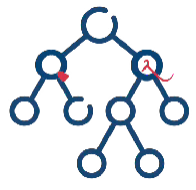
\includegraphics[height=0.9cm]{msca_logo.png}}%
  \end{center}
  \vspace{0.45cm}
  \begin{center}
    \begin{minipage}{0.1\textwidth}\centering
      \href{https://quantlet.com}{
\includegraphics[height=0.9cm]{ql_logo.png}}\end{minipage}%
    \begin{minipage}{0.78\textwidth}\centering
      {\Large\bfseries\usebeamercolor[fg]{title}\inserttitle}\par\vspace{0.25cm}
      {\large\usebeamercolor[fg]{title}\insertsubtitle}\end{minipage}%
    \begin{minipage}{0.1\textwidth}\centering
      \href{https://quantinar.com}{
\includegraphics[height=0.9cm]{qr_logo.png}}\end{minipage}
  \end{center}
  \vfill
  \hspace{0.4cm}{\bfseries\insertauthor}\par\vspace{0.12cm}
  \hspace{0.4cm}\begin{minipage}[t]{0.92\textwidth}\raggedright\footnotesize\insertinstitute\end{minipage}
  \par\vspace{0.4cm}}

% ---------------------------------------------------------------- lecture metadata
\newcommand{\nnshort}{}
\newcommand{\nnnb}{notebooks}
\newcommand{\nnrepo}{https://github.com/danpele/NEURAL_BIZ/tree/main}
% language-dependent labels (English default; \nnromanian switches to Romanian, call it before \nnlecture)
\newcommand{\txtcourse}{Neural Networks and Deep Learning}
\newcommand{\txtlecture}{Lecture}
\newcommand{\txtoutline}{Outline}
\newcommand{\txtintuition}{In one sentence:}
\newcommand{\txtjob}{In practice:}
\newcommand{\txttry}{Experiment yourself:}
\newcommand{\txtwhere}{where}
\newcommand{\txtsim}{SIMULATED DATA (teaching illustration)}
\newcommand{\txtnbsuffix}{}
\newcommand{\txtinstitute}{Bucharest University of Economic Studies (ASE), Department of Statistics and Econometrics\\
    Romanian Academy, Institute for Economic Forecasting (IPE)\\
    IDA Institute Digital Assets \textbullet\ AI4EFin \textbullet\ MSCA Digital Finance}
\newcommand{\nnromanian}{%
  \renewcommand{\txtcourse}{Rețele neuronale și deep learning}%
  \renewcommand{\txtlecture}{Cursul}%
  \renewcommand{\txtoutline}{Cuprins}%
  \renewcommand{\txtintuition}{Pe scurt:}%
  \renewcommand{\txtjob}{În practică:}%
  \renewcommand{\txttry}{Exercițiu practic:}%
  \renewcommand{\txtwhere}{unde}%
  \renewcommand{\txtsim}{DATE SIMULATE (doar pentru ilustrare)}%
  \renewcommand{\txtnbsuffix}{\string_ro}%
  \renewcommand{\txtinstitute}{Academia de Studii Economice din București (ASE), Departamentul de Statistică și Econometrie\\
    Academia Română, Institutul de Prognoză Economică (IPE)\\
    IDA Institute Digital Assets \textbullet\ AI4EFin \textbullet\ MSCA Digital Finance}}
\newcommand{\nnlecture}[2]{%
  \renewcommand{\nnshort}{\txtlecture\ #1}%
  \renewcommand{\nnnb}{notebooks/L#1\string_notebook\txtnbsuffix.ipynb}%
  \title[NN]{\txtcourse}%
  \subtitle{\txtlecture\ #1: #2}%
  \author{Prof.\ dr.\ Daniel Traian PELE}%
  \institute{\txtinstitute}%
  \date{}}

% ---------------------------------------------------------------- teaching blocks (one message per frame)
% \intuition{one plain sentence}  ->  formula with every symbol defined  ->  real-data example  ->  \manager{one line}
\newcommand{\intuition}[1]{\begin{itemize}\item {\color{MainBlue}\textbf{\txtintuition}}~#1\end{itemize}\vspace{0.6mm}}
\newcommand{\manager}[1]{\colorbox{Forest!10}{\parbox{\dimexpr\linewidth-2\fboxsep\relax}{\footnotesize
  \begin{itemize}\setlength{\itemsep}{0pt}\item \textbf{\color{Forest}\txtjob}~#1\end{itemize}}}}
% Experiment yourself: pointer to the matching notebook section
\newcommand{\tryit}[1]{{\scriptsize\href{\nnrepo/\nnnb}{%
  \raisebox{-0.15em}{
\includegraphics[height=0.85em]{ql_logo.png}}\,\textbf{\txttry}~\color{MainBlue}#1}}}
% bottom row: manager line (left) + experiment pointer (right), pinned to the bottom of the frame
\newcommand{\bottomrow}[2]{\par\vfill\noindent\begin{minipage}[b]{0.72\linewidth}#1\end{minipage}\hfill
  \begin{minipage}[b]{0.26\linewidth}\raggedleft #2\end{minipage}\par\vspace{0.5mm}}
\newcommand{\where}[1]{{\footnotesize\textbf{\txtwhere}~#1\par}}

% ---------------------------------------------------------------- helpers
% chart source line under a figure: \chartsource{Source ...; period ...}
\newcommand{\chartsource}[1]{\par\vspace{1pt}{\scriptsize\color{FooterGray}#1\par}}
% link to code: \quantlet{label}{path inside the repo}
\newcommand{\quantlet}[2]{\par\vspace{1pt}\hfill\href{\nnrepo/#2}{%
  \raisebox{-0.15em}{
\includegraphics[height=0.75em]{ql_logo.png}}\textcolor{MainBlue}{\scriptsize\ #1}}}
% inline Quantlet link for the bottom-right corner of a frame: \qlink{label}{path inside the repo}
\newcommand{\qlink}[2]{{\scriptsize\href{\nnrepo/#2}{\raisebox{-0.15em}{
\includegraphics[height=0.85em]{ql_logo.png}}\,\textcolor{MainBlue}{#1}}}}
\newcommand{\simlabel}{\colorbox{Crimson!12}{\scriptsize\bfseries\color{Crimson}\txtsim}}
\newcommand{\E}{\mathbb{E}}
\newcommand{\Var}{\operatorname{Var}}
\newcommand{\Cov}{\operatorname{Cov}}
\newcommand{\Corr}{\operatorname{Corr}}
\newcommand{\asinh}{\operatorname{asinh}}
\newcommand{\iid}{\overset{\text{i.i.d.}}{\sim}}
\newcommand{\EUR}{EUR}
% deep-learning notation (Bishop & Bishop, 2024): vectors bold lower case, matrices bold upper case
\newcommand{\R}{\mathbb{R}}
\newcommand{\vx}{\mathbf{x}}
\newcommand{\vy}{\mathbf{y}}
\newcommand{\vz}{\mathbf{z}}
\newcommand{\vh}{\mathbf{h}}
\newcommand{\vw}{\mathbf{w}}
\newcommand{\vb}{\mathbf{b}}
\newcommand{\mW}{\mathbf{W}}
\newcommand{\mX}{\mathbf{X}}
\newcommand{\btheta}{\boldsymbol{\theta}}
\newcommand{\loss}{\mathcal{L}}
\newcommand{\dataset}{\mathcal{D}}
\DeclareMathOperator*{\argmin}{arg\,min}
\DeclareMathOperator*{\argmax}{arg\,max}
\DeclareMathOperator{\softmax}{softmax}
\DeclareMathOperator{\ReLU}{ReLU}
\DeclareMathOperator{\sigm}{\sigma}

%   \nnlecture{k}{Lecture title}
% Logos live in lectures/common/logos/, charts in lectures/Lk/charts/.
% Do NOT add \hfuzz / \vfuzz / \hbadness here: overfull boxes must be fixed, not hidden.
% =============================================================================

\usetheme{default}
\setbeamersize{text margin left=7mm, text margin right=7mm}

% ---------------------------------------------------------------- packages
\usepackage[utf8]{inputenc}
\usepackage[T1]{fontenc}
\usepackage{lmodern}
\usepackage{amsmath, amssymb}
\usepackage{mathtools}
\usepackage{bm}
\usepackage{tikz}
\usetikzlibrary{arrows.meta, positioning, calc, shapes.misc}
\usepackage{booktabs}
\usepackage{array}
\usepackage{graphicx}
\usepackage{colortbl}
\usepackage{xcolor}
\usepackage{multicol}
\hypersetup{colorlinks=true, linkcolor=MainBlue, urlcolor=MainBlue, citecolor=MainBlue}
\graphicspath{{../common/logos/}}   % charts are included with their language folder: charts/en/, charts/ro/

% ---------------------------------------------------------------- colours
\definecolor{MainBlue}{RGB}{26, 58, 110}
\definecolor{IDAred}{RGB}{205, 0, 0}
\definecolor{DarkGray}{RGB}{51, 51, 51}
\definecolor{FooterGray}{RGB}{100, 100, 100}
\definecolor{BlockGray}{RGB}{236, 238, 242}
\definecolor{KeynoteGray}{RGB}{218, 218, 218}
\definecolor{Crimson}{RGB}{190, 40, 50}
\definecolor{Forest}{RGB}{30, 110, 50}
\definecolor{Bitter}{RGB}{214, 150, 20}
% chart palette (same hex values and order as lectures/common/nn_plot.py SERIES)
\definecolor{Ser1}{HTML}{2A78D6}
\definecolor{Ser2}{HTML}{EB6834}
\definecolor{Ser3}{HTML}{1BAF7A}
\definecolor{Ser4}{HTML}{EDA100}
\definecolor{Ser5}{HTML}{E87BA4}
\definecolor{Ser6}{HTML}{008300}
\definecolor{Ser7}{HTML}{6250D6}
\definecolor{Ser8}{HTML}{E34948}

\setbeamertemplate{background}{%
  \begin{tikzpicture}[remember picture, overlay]
    \shade[shading=axis, shading angle=315, top color=white, bottom color=KeynoteGray]
      (current page.south west) rectangle (current page.north east);
  \end{tikzpicture}}
\setbeamercolor{background canvas}{bg=}
\setbeamercolor{structure}{fg=MainBlue}
\setbeamercolor{normal text}{fg=DarkGray}
\setbeamercolor{title}{fg=IDAred}
\setbeamercolor{frametitle}{fg=IDAred, bg=}
\setbeamercolor{block title}{bg=MainBlue, fg=white}
\setbeamercolor{block body}{bg=BlockGray, fg=DarkGray}
\setbeamercolor{block title alerted}{bg=Crimson, fg=white}
\setbeamercolor{block body alerted}{bg=Crimson!7, fg=DarkGray}
\setbeamercolor{block title example}{bg=Forest, fg=white}
\setbeamercolor{block body example}{bg=Forest!7, fg=DarkGray}
\setbeamercolor{item}{fg=MainBlue}
\setbeamerfont{frametitle}{size=\large, series=\bfseries}
\setbeamerfont{block title}{size=\small, series=\bfseries}
\setbeamertemplate{blocks}[rounded][shadow=false]
\setbeamertemplate{itemize item}{\color{MainBlue}$\boxdot$}
\setbeamertemplate{itemize subitem}{\color{MainBlue}\scriptsize$\blacktriangleright$}
% compact two-level lists: level 1 = main point, level 2 = details (no text outside bullets)
\setbeamerfont{itemize/enumerate subbody}{size=\footnotesize}
\setlength{\leftmargini}{1.1em}
\setlength{\leftmarginii}{1.1em}
\setbeamertemplate{itemize/enumerate body begin}{\setlength{\topsep}{0pt}\setlength{\partopsep}{0pt}\setlength{\parskip}{0pt}}
\setbeamertemplate{itemize/enumerate subbody begin}{\setlength{\topsep}{0pt}\setlength{\partopsep}{0pt}\setlength{\itemsep}{0pt}\vspace{-0.4ex}}

\setbeamertemplate{enumerate item}{\color{MainBlue}\insertenumlabel.}
\setlength{\leftmargini}{1.3em}
\setlength{\leftmarginii}{1.2em}
\setbeamertemplate{navigation symbols}{}
\setbeamertemplate{section in toc}{\color{MainBlue}$\blacktriangleright$~\inserttocsection}
\setbeamertemplate{caption}{\raggedright\insertcaption\par}
% frame subtitle = precise citation line under the claim title (Weron style)
\setbeamerfont{framesubtitle}{size=\footnotesize}
\setbeamercolor{framesubtitle}{fg=FooterGray}
% outline that reappears at every section with the current section highlighted
\setbeamertemplate{section in toc shaded}[default][35]
\setbeamertemplate{subsection in toc shaded}[default][35]
\setbeamertemplate{subsection in toc}{\leavevmode\leftskip=2.2em\color{DarkGray}\small\inserttocsubsection\par}
\AtBeginSection[]{{\begin{frame}{\txtoutline}\vspace{2mm}\small
  \tableofcontents[currentsection,hideothersubsections]\end{frame}}}

% ---------------------------------------------------------------- head and foot
\setbeamertemplate{headline}{%
  \vskip10pt%
  \hbox to \paperwidth{\hskip0.5cm%
    {\small\color{FooterGray}\renewcommand{\hyperlink}[2]{##2}\insertsectionhead}%
    \hfill\textcolor{FooterGray}{\small\insertframenumber}\hskip0.5cm}%
  \vskip4pt{\color{FooterGray}\hrule height 0.4pt}}
% footer as in the other courses (MFM, SFM): course name on the left, small sparkline on the right
\setbeamertemplate{footline}{%
  {\color{FooterGray}\hrule height 0.4pt}\vskip4pt%
  \hbox to \paperwidth{\hskip0.5cm%
    \textcolor{FooterGray}{\small\txtcourse}%
    \hfill\raisebox{-0.1em}{\begin{tikzpicture}[x=0.08em, y=0.08em, line width=0.4pt]
      \draw[FooterGray] (0,3) -- (1,4) -- (2,3.5) -- (3,5) -- (4,4) -- (5,6) -- (6,5.5) -- (7,4) -- (8,5) -- (9,7) -- (10,6) -- (11,5) -- (12,6.5) -- (13,8) -- (14,7) -- (15,6) -- (16,7.5) -- (17,9) -- (18,8) -- (19,7) -- (20,8.5) -- (21,10) -- (22,9) -- (23,8) -- (24,9.5);
    \end{tikzpicture}}\hskip0.5cm}%
  \vskip6pt}

% ---------------------------------------------------------------- title page
\defbeamertemplate*{title page}{nn}[1][]{%
  \vspace{0.15cm}
  \begin{center}
    \href{https://www.ase.ro}{
\includegraphics[height=0.9cm]{ase_logo.png}}\hspace{0.3cm}%
    \href{https://ipe.ro/new}{
\includegraphics[height=0.9cm]{acad_logo.png}}\hspace{0.3cm}%
    \href{https://theida.net}{
\includegraphics[height=0.9cm]{ida_logo.png}}\hspace{0.3cm}%
    \href{https://blockchain-research-center.com}{
\includegraphics[height=0.9cm]{brc_logo.png}}\hspace{0.3cm}%
    \href{https://www.ai4efin.ase.ro}{
\includegraphics[height=0.9cm]{ai4efin_logo.png}}\hspace{0.3cm}%
    \href{https://www.digital-finance-msca.com}{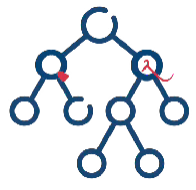
\includegraphics[height=0.9cm]{msca_logo.png}}%
  \end{center}
  \vspace{0.45cm}
  \begin{center}
    \begin{minipage}{0.1\textwidth}\centering
      \href{https://quantlet.com}{
\includegraphics[height=0.9cm]{ql_logo.png}}\end{minipage}%
    \begin{minipage}{0.78\textwidth}\centering
      {\Large\bfseries\usebeamercolor[fg]{title}\inserttitle}\par\vspace{0.25cm}
      {\large\usebeamercolor[fg]{title}\insertsubtitle}\end{minipage}%
    \begin{minipage}{0.1\textwidth}\centering
      \href{https://quantinar.com}{
\includegraphics[height=0.9cm]{qr_logo.png}}\end{minipage}
  \end{center}
  \vfill
  \hspace{0.4cm}{\bfseries\insertauthor}\par\vspace{0.12cm}
  \hspace{0.4cm}\begin{minipage}[t]{0.92\textwidth}\raggedright\footnotesize\insertinstitute\end{minipage}
  \par\vspace{0.4cm}}

% ---------------------------------------------------------------- lecture metadata
\newcommand{\nnshort}{}
\newcommand{\nnnb}{notebooks}
\newcommand{\nnrepo}{https://github.com/danpele/NEURAL_BIZ/tree/main}
% language-dependent labels (English default; \nnromanian switches to Romanian, call it before \nnlecture)
\newcommand{\txtcourse}{Neural Networks and Deep Learning}
\newcommand{\txtlecture}{Lecture}
\newcommand{\txtoutline}{Outline}
\newcommand{\txtintuition}{In one sentence:}
\newcommand{\txtjob}{In practice:}
\newcommand{\txttry}{Experiment yourself:}
\newcommand{\txtwhere}{where}
\newcommand{\txtsim}{SIMULATED DATA (teaching illustration)}
\newcommand{\txtnbsuffix}{}
\newcommand{\txtinstitute}{Bucharest University of Economic Studies (ASE), Department of Statistics and Econometrics\\
    Romanian Academy, Institute for Economic Forecasting (IPE)\\
    IDA Institute Digital Assets \textbullet\ AI4EFin \textbullet\ MSCA Digital Finance}
\newcommand{\nnromanian}{%
  \renewcommand{\txtcourse}{Rețele neuronale și deep learning}%
  \renewcommand{\txtlecture}{Cursul}%
  \renewcommand{\txtoutline}{Cuprins}%
  \renewcommand{\txtintuition}{Pe scurt:}%
  \renewcommand{\txtjob}{În practică:}%
  \renewcommand{\txttry}{Exercițiu practic:}%
  \renewcommand{\txtwhere}{unde}%
  \renewcommand{\txtsim}{DATE SIMULATE (doar pentru ilustrare)}%
  \renewcommand{\txtnbsuffix}{\string_ro}%
  \renewcommand{\txtinstitute}{Academia de Studii Economice din București (ASE), Departamentul de Statistică și Econometrie\\
    Academia Română, Institutul de Prognoză Economică (IPE)\\
    IDA Institute Digital Assets \textbullet\ AI4EFin \textbullet\ MSCA Digital Finance}}
\newcommand{\nnlecture}[2]{%
  \renewcommand{\nnshort}{\txtlecture\ #1}%
  \renewcommand{\nnnb}{notebooks/L#1\string_notebook\txtnbsuffix.ipynb}%
  \title[NN]{\txtcourse}%
  \subtitle{\txtlecture\ #1: #2}%
  \author{Prof.\ dr.\ Daniel Traian PELE}%
  \institute{\txtinstitute}%
  \date{}}

% ---------------------------------------------------------------- teaching blocks (one message per frame)
% \intuition{one plain sentence}  ->  formula with every symbol defined  ->  real-data example  ->  \manager{one line}
\newcommand{\intuition}[1]{\begin{itemize}\item {\color{MainBlue}\textbf{\txtintuition}}~#1\end{itemize}\vspace{0.6mm}}
\newcommand{\manager}[1]{\colorbox{Forest!10}{\parbox{\dimexpr\linewidth-2\fboxsep\relax}{\footnotesize
  \begin{itemize}\setlength{\itemsep}{0pt}\item \textbf{\color{Forest}\txtjob}~#1\end{itemize}}}}
% Experiment yourself: pointer to the matching notebook section
\newcommand{\tryit}[1]{{\scriptsize\href{\nnrepo/\nnnb}{%
  \raisebox{-0.15em}{
\includegraphics[height=0.85em]{ql_logo.png}}\,\textbf{\txttry}~\color{MainBlue}#1}}}
% bottom row: manager line (left) + experiment pointer (right), pinned to the bottom of the frame
\newcommand{\bottomrow}[2]{\par\vfill\noindent\begin{minipage}[b]{0.72\linewidth}#1\end{minipage}\hfill
  \begin{minipage}[b]{0.26\linewidth}\raggedleft #2\end{minipage}\par\vspace{0.5mm}}
\newcommand{\where}[1]{{\footnotesize\textbf{\txtwhere}~#1\par}}

% ---------------------------------------------------------------- helpers
% chart source line under a figure: \chartsource{Source ...; period ...}
\newcommand{\chartsource}[1]{\par\vspace{1pt}{\scriptsize\color{FooterGray}#1\par}}
% link to code: \quantlet{label}{path inside the repo}
\newcommand{\quantlet}[2]{\par\vspace{1pt}\hfill\href{\nnrepo/#2}{%
  \raisebox{-0.15em}{
\includegraphics[height=0.75em]{ql_logo.png}}\textcolor{MainBlue}{\scriptsize\ #1}}}
% inline Quantlet link for the bottom-right corner of a frame: \qlink{label}{path inside the repo}
\newcommand{\qlink}[2]{{\scriptsize\href{\nnrepo/#2}{\raisebox{-0.15em}{
\includegraphics[height=0.85em]{ql_logo.png}}\,\textcolor{MainBlue}{#1}}}}
\newcommand{\simlabel}{\colorbox{Crimson!12}{\scriptsize\bfseries\color{Crimson}\txtsim}}
\newcommand{\E}{\mathbb{E}}
\newcommand{\Var}{\operatorname{Var}}
\newcommand{\Cov}{\operatorname{Cov}}
\newcommand{\Corr}{\operatorname{Corr}}
\newcommand{\asinh}{\operatorname{asinh}}
\newcommand{\iid}{\overset{\text{i.i.d.}}{\sim}}
\newcommand{\EUR}{EUR}
% deep-learning notation (Bishop & Bishop, 2024): vectors bold lower case, matrices bold upper case
\newcommand{\R}{\mathbb{R}}
\newcommand{\vx}{\mathbf{x}}
\newcommand{\vy}{\mathbf{y}}
\newcommand{\vz}{\mathbf{z}}
\newcommand{\vh}{\mathbf{h}}
\newcommand{\vw}{\mathbf{w}}
\newcommand{\vb}{\mathbf{b}}
\newcommand{\mW}{\mathbf{W}}
\newcommand{\mX}{\mathbf{X}}
\newcommand{\btheta}{\boldsymbol{\theta}}
\newcommand{\loss}{\mathcal{L}}
\newcommand{\dataset}{\mathcal{D}}
\DeclareMathOperator*{\argmin}{arg\,min}
\DeclareMathOperator*{\argmax}{arg\,max}
\DeclareMathOperator{\softmax}{softmax}
\DeclareMathOperator{\ReLU}{ReLU}
\DeclareMathOperator{\sigm}{\sigma}

%   \nnlecture{k}{Lecture title}
% Logos live in lectures/common/logos/, charts in lectures/Lk/charts/.
% Do NOT add \hfuzz / \vfuzz / \hbadness here: overfull boxes must be fixed, not hidden.
% =============================================================================

\usetheme{default}
\setbeamersize{text margin left=7mm, text margin right=7mm}

% ---------------------------------------------------------------- packages
\usepackage[utf8]{inputenc}
\usepackage[T1]{fontenc}
\usepackage{lmodern}
\usepackage{amsmath, amssymb}
\usepackage{mathtools}
\usepackage{bm}
\usepackage{tikz}
\usetikzlibrary{arrows.meta, positioning, calc, shapes.misc}
\usepackage{booktabs}
\usepackage{array}
\usepackage{graphicx}
\usepackage{colortbl}
\usepackage{xcolor}
\usepackage{multicol}
\hypersetup{colorlinks=true, linkcolor=MainBlue, urlcolor=MainBlue, citecolor=MainBlue}
\graphicspath{{../common/logos/}}   % charts are included with their language folder: charts/en/, charts/ro/

% ---------------------------------------------------------------- colours
\definecolor{MainBlue}{RGB}{26, 58, 110}
\definecolor{IDAred}{RGB}{205, 0, 0}
\definecolor{DarkGray}{RGB}{51, 51, 51}
\definecolor{FooterGray}{RGB}{100, 100, 100}
\definecolor{BlockGray}{RGB}{236, 238, 242}
\definecolor{KeynoteGray}{RGB}{218, 218, 218}
\definecolor{Crimson}{RGB}{190, 40, 50}
\definecolor{Forest}{RGB}{30, 110, 50}
\definecolor{Bitter}{RGB}{214, 150, 20}
% chart palette (same hex values and order as lectures/common/nn_plot.py SERIES)
\definecolor{Ser1}{HTML}{2A78D6}
\definecolor{Ser2}{HTML}{EB6834}
\definecolor{Ser3}{HTML}{1BAF7A}
\definecolor{Ser4}{HTML}{EDA100}
\definecolor{Ser5}{HTML}{E87BA4}
\definecolor{Ser6}{HTML}{008300}
\definecolor{Ser7}{HTML}{6250D6}
\definecolor{Ser8}{HTML}{E34948}

\setbeamertemplate{background}{%
  \begin{tikzpicture}[remember picture, overlay]
    \shade[shading=axis, shading angle=315, top color=white, bottom color=KeynoteGray]
      (current page.south west) rectangle (current page.north east);
  \end{tikzpicture}}
\setbeamercolor{background canvas}{bg=}
\setbeamercolor{structure}{fg=MainBlue}
\setbeamercolor{normal text}{fg=DarkGray}
\setbeamercolor{title}{fg=IDAred}
\setbeamercolor{frametitle}{fg=IDAred, bg=}
\setbeamercolor{block title}{bg=MainBlue, fg=white}
\setbeamercolor{block body}{bg=BlockGray, fg=DarkGray}
\setbeamercolor{block title alerted}{bg=Crimson, fg=white}
\setbeamercolor{block body alerted}{bg=Crimson!7, fg=DarkGray}
\setbeamercolor{block title example}{bg=Forest, fg=white}
\setbeamercolor{block body example}{bg=Forest!7, fg=DarkGray}
\setbeamercolor{item}{fg=MainBlue}
\setbeamerfont{frametitle}{size=\large, series=\bfseries}
\setbeamerfont{block title}{size=\small, series=\bfseries}
\setbeamertemplate{blocks}[rounded][shadow=false]
\setbeamertemplate{itemize item}{\color{MainBlue}$\boxdot$}
\setbeamertemplate{itemize subitem}{\color{MainBlue}\scriptsize$\blacktriangleright$}
% compact two-level lists: level 1 = main point, level 2 = details (no text outside bullets)
\setbeamerfont{itemize/enumerate subbody}{size=\footnotesize}
\setlength{\leftmargini}{1.1em}
\setlength{\leftmarginii}{1.1em}
\setbeamertemplate{itemize/enumerate body begin}{\setlength{\topsep}{0pt}\setlength{\partopsep}{0pt}\setlength{\parskip}{0pt}}
\setbeamertemplate{itemize/enumerate subbody begin}{\setlength{\topsep}{0pt}\setlength{\partopsep}{0pt}\setlength{\itemsep}{0pt}\vspace{-0.4ex}}

\setbeamertemplate{enumerate item}{\color{MainBlue}\insertenumlabel.}
\setlength{\leftmargini}{1.3em}
\setlength{\leftmarginii}{1.2em}
\setbeamertemplate{navigation symbols}{}
\setbeamertemplate{section in toc}{\color{MainBlue}$\blacktriangleright$~\inserttocsection}
\setbeamertemplate{caption}{\raggedright\insertcaption\par}
% frame subtitle = precise citation line under the claim title (Weron style)
\setbeamerfont{framesubtitle}{size=\footnotesize}
\setbeamercolor{framesubtitle}{fg=FooterGray}
% outline that reappears at every section with the current section highlighted
\setbeamertemplate{section in toc shaded}[default][35]
\setbeamertemplate{subsection in toc shaded}[default][35]
\setbeamertemplate{subsection in toc}{\leavevmode\leftskip=2.2em\color{DarkGray}\small\inserttocsubsection\par}
\AtBeginSection[]{{\begin{frame}{\txtoutline}\vspace{2mm}\small
  \tableofcontents[currentsection,hideothersubsections]\end{frame}}}

% ---------------------------------------------------------------- head and foot
\setbeamertemplate{headline}{%
  \vskip10pt%
  \hbox to \paperwidth{\hskip0.5cm%
    {\small\color{FooterGray}\renewcommand{\hyperlink}[2]{##2}\insertsectionhead}%
    \hfill\textcolor{FooterGray}{\small\insertframenumber}\hskip0.5cm}%
  \vskip4pt{\color{FooterGray}\hrule height 0.4pt}}
% footer as in the other courses (MFM, SFM): course name on the left, small sparkline on the right
\setbeamertemplate{footline}{%
  {\color{FooterGray}\hrule height 0.4pt}\vskip4pt%
  \hbox to \paperwidth{\hskip0.5cm%
    \textcolor{FooterGray}{\small\txtcourse}%
    \hfill\raisebox{-0.1em}{\begin{tikzpicture}[x=0.08em, y=0.08em, line width=0.4pt]
      \draw[FooterGray] (0,3) -- (1,4) -- (2,3.5) -- (3,5) -- (4,4) -- (5,6) -- (6,5.5) -- (7,4) -- (8,5) -- (9,7) -- (10,6) -- (11,5) -- (12,6.5) -- (13,8) -- (14,7) -- (15,6) -- (16,7.5) -- (17,9) -- (18,8) -- (19,7) -- (20,8.5) -- (21,10) -- (22,9) -- (23,8) -- (24,9.5);
    \end{tikzpicture}}\hskip0.5cm}%
  \vskip6pt}

% ---------------------------------------------------------------- title page
\defbeamertemplate*{title page}{nn}[1][]{%
  \vspace{0.15cm}
  \begin{center}
    \href{https://www.ase.ro}{
\includegraphics[height=0.9cm]{ase_logo.png}}\hspace{0.3cm}%
    \href{https://ipe.ro/new}{
\includegraphics[height=0.9cm]{acad_logo.png}}\hspace{0.3cm}%
    \href{https://theida.net}{
\includegraphics[height=0.9cm]{ida_logo.png}}\hspace{0.3cm}%
    \href{https://blockchain-research-center.com}{
\includegraphics[height=0.9cm]{brc_logo.png}}\hspace{0.3cm}%
    \href{https://www.ai4efin.ase.ro}{
\includegraphics[height=0.9cm]{ai4efin_logo.png}}\hspace{0.3cm}%
    \href{https://www.digital-finance-msca.com}{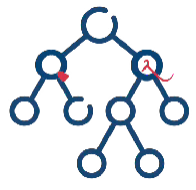
\includegraphics[height=0.9cm]{msca_logo.png}}%
  \end{center}
  \vspace{0.45cm}
  \begin{center}
    \begin{minipage}{0.1\textwidth}\centering
      \href{https://quantlet.com}{
\includegraphics[height=0.9cm]{ql_logo.png}}\end{minipage}%
    \begin{minipage}{0.78\textwidth}\centering
      {\Large\bfseries\usebeamercolor[fg]{title}\inserttitle}\par\vspace{0.25cm}
      {\large\usebeamercolor[fg]{title}\insertsubtitle}\end{minipage}%
    \begin{minipage}{0.1\textwidth}\centering
      \href{https://quantinar.com}{
\includegraphics[height=0.9cm]{qr_logo.png}}\end{minipage}
  \end{center}
  \vfill
  \hspace{0.4cm}{\bfseries\insertauthor}\par\vspace{0.12cm}
  \hspace{0.4cm}\begin{minipage}[t]{0.92\textwidth}\raggedright\footnotesize\insertinstitute\end{minipage}
  \par\vspace{0.4cm}}

% ---------------------------------------------------------------- lecture metadata
\newcommand{\nnshort}{}
\newcommand{\nnnb}{notebooks}
\newcommand{\nnrepo}{https://github.com/danpele/NEURAL_BIZ/tree/main}
% language-dependent labels (English default; \nnromanian switches to Romanian, call it before \nnlecture)
\newcommand{\txtcourse}{Neural Networks and Deep Learning}
\newcommand{\txtlecture}{Lecture}
\newcommand{\txtoutline}{Outline}
\newcommand{\txtintuition}{In one sentence:}
\newcommand{\txtjob}{In practice:}
\newcommand{\txttry}{Experiment yourself:}
\newcommand{\txtwhere}{where}
\newcommand{\txtsim}{SIMULATED DATA (teaching illustration)}
\newcommand{\txtnbsuffix}{}
\newcommand{\txtinstitute}{Bucharest University of Economic Studies (ASE), Department of Statistics and Econometrics\\
    Romanian Academy, Institute for Economic Forecasting (IPE)\\
    IDA Institute Digital Assets \textbullet\ AI4EFin \textbullet\ MSCA Digital Finance}
\newcommand{\nnromanian}{%
  \renewcommand{\txtcourse}{Rețele neuronale și deep learning}%
  \renewcommand{\txtlecture}{Cursul}%
  \renewcommand{\txtoutline}{Cuprins}%
  \renewcommand{\txtintuition}{Pe scurt:}%
  \renewcommand{\txtjob}{În practică:}%
  \renewcommand{\txttry}{Exercițiu practic:}%
  \renewcommand{\txtwhere}{unde}%
  \renewcommand{\txtsim}{DATE SIMULATE (doar pentru ilustrare)}%
  \renewcommand{\txtnbsuffix}{\string_ro}%
  \renewcommand{\txtinstitute}{Academia de Studii Economice din București (ASE), Departamentul de Statistică și Econometrie\\
    Academia Română, Institutul de Prognoză Economică (IPE)\\
    IDA Institute Digital Assets \textbullet\ AI4EFin \textbullet\ MSCA Digital Finance}}
\newcommand{\nnlecture}[2]{%
  \renewcommand{\nnshort}{\txtlecture\ #1}%
  \renewcommand{\nnnb}{notebooks/L#1\string_notebook\txtnbsuffix.ipynb}%
  \title[NN]{\txtcourse}%
  \subtitle{\txtlecture\ #1: #2}%
  \author{Prof.\ dr.\ Daniel Traian PELE}%
  \institute{\txtinstitute}%
  \date{}}

% ---------------------------------------------------------------- teaching blocks (one message per frame)
% \intuition{one plain sentence}  ->  formula with every symbol defined  ->  real-data example  ->  \manager{one line}
\newcommand{\intuition}[1]{\begin{itemize}\item {\color{MainBlue}\textbf{\txtintuition}}~#1\end{itemize}\vspace{0.6mm}}
\newcommand{\manager}[1]{\colorbox{Forest!10}{\parbox{\dimexpr\linewidth-2\fboxsep\relax}{\footnotesize
  \begin{itemize}\setlength{\itemsep}{0pt}\item \textbf{\color{Forest}\txtjob}~#1\end{itemize}}}}
% Experiment yourself: pointer to the matching notebook section
\newcommand{\tryit}[1]{{\scriptsize\href{\nnrepo/\nnnb}{%
  \raisebox{-0.15em}{
\includegraphics[height=0.85em]{ql_logo.png}}\,\textbf{\txttry}~\color{MainBlue}#1}}}
% bottom row: manager line (left) + experiment pointer (right), pinned to the bottom of the frame
\newcommand{\bottomrow}[2]{\par\vfill\noindent\begin{minipage}[b]{0.72\linewidth}#1\end{minipage}\hfill
  \begin{minipage}[b]{0.26\linewidth}\raggedleft #2\end{minipage}\par\vspace{0.5mm}}
\newcommand{\where}[1]{{\footnotesize\textbf{\txtwhere}~#1\par}}

% ---------------------------------------------------------------- helpers
% chart source line under a figure: \chartsource{Source ...; period ...}
\newcommand{\chartsource}[1]{\par\vspace{1pt}{\scriptsize\color{FooterGray}#1\par}}
% link to code: \quantlet{label}{path inside the repo}
\newcommand{\quantlet}[2]{\par\vspace{1pt}\hfill\href{\nnrepo/#2}{%
  \raisebox{-0.15em}{
\includegraphics[height=0.75em]{ql_logo.png}}\textcolor{MainBlue}{\scriptsize\ #1}}}
% inline Quantlet link for the bottom-right corner of a frame: \qlink{label}{path inside the repo}
\newcommand{\qlink}[2]{{\scriptsize\href{\nnrepo/#2}{\raisebox{-0.15em}{
\includegraphics[height=0.85em]{ql_logo.png}}\,\textcolor{MainBlue}{#1}}}}
\newcommand{\simlabel}{\colorbox{Crimson!12}{\scriptsize\bfseries\color{Crimson}\txtsim}}
\newcommand{\E}{\mathbb{E}}
\newcommand{\Var}{\operatorname{Var}}
\newcommand{\Cov}{\operatorname{Cov}}
\newcommand{\Corr}{\operatorname{Corr}}
\newcommand{\asinh}{\operatorname{asinh}}
\newcommand{\iid}{\overset{\text{i.i.d.}}{\sim}}
\newcommand{\EUR}{EUR}
% deep-learning notation (Bishop & Bishop, 2024): vectors bold lower case, matrices bold upper case
\newcommand{\R}{\mathbb{R}}
\newcommand{\vx}{\mathbf{x}}
\newcommand{\vy}{\mathbf{y}}
\newcommand{\vz}{\mathbf{z}}
\newcommand{\vh}{\mathbf{h}}
\newcommand{\vw}{\mathbf{w}}
\newcommand{\vb}{\mathbf{b}}
\newcommand{\mW}{\mathbf{W}}
\newcommand{\mX}{\mathbf{X}}
\newcommand{\btheta}{\boldsymbol{\theta}}
\newcommand{\loss}{\mathcal{L}}
\newcommand{\dataset}{\mathcal{D}}
\DeclareMathOperator*{\argmin}{arg\,min}
\DeclareMathOperator*{\argmax}{arg\,max}
\DeclareMathOperator{\softmax}{softmax}
\DeclareMathOperator{\ReLU}{ReLU}
\DeclareMathOperator{\sigm}{\sigma}

\nnlecture{7}{Attention and transformers}
\begin{document}
{\setbeamertemplate{headline}{}\setbeamertemplate{footline}{}
\begin{frame}\titlepage\end{frame}}
% END-FRONT-MATTER

\begin{frame}{Learning objectives}
\small
\begin{itemize}\setlength{\itemsep}{5pt}
  \item Explain why attention replaced recurrence for text: one step between any two words, computed in parallel.
  \item Write scaled dot-product attention, multi-head attention, positional encoding and the transformer block with every symbol defined.
  \item Compare, on real finance tweets, a small transformer trained from scratch, a pretrained Bidirectional Encoder Representations from Transformers (BERT) model for finance (FinBERT) and a term frequency--inverse document frequency (TF-IDF) benchmark.
  \item Read attention maps with care, and decide when pretraining, fine-tuning or a simple model is the right business choice.
\end{itemize}
\end{frame}

% BEGIN-ABBR

\begin{frame}{Abbreviations}
\small
\vspace{-1mm}\begin{columns}[T,onlytextwidth]
\begin{column}{0.49\textwidth}{\scriptsize\renewcommand{\arraystretch}{0.96}\begin{tabular}{@{}>{\bfseries}l@{\ \ }p{0.74\linewidth}@{}}ASE & Bucharest University of Economic Studies\\
BERT & Bidirectional Encoder Representations from Transformers\\
CNN & convolutional neural network\\
ECB & European Central Bank\\
ES & expected shortfall\\
FFN & position-wise feed-forward network\\
FinBERT & BERT further trained on financial text\\
GELU & Gaussian error linear unit\\
GPT & Generative Pre-trained Transformer\\
IPE & Institute for Economic Forecasting, Romanian Academy\\
LLM & large language model\\\end{tabular}}\end{column}
\begin{column}{0.49\textwidth}{\scriptsize\renewcommand{\arraystretch}{0.96}\begin{tabular}{@{}>{\bfseries}l@{\ \ }p{0.74\linewidth}@{}}LN & layer normalisation\\
LSTM & long short-term memory network\\
MHA & multi-head attention\\
MLM & masked language modelling\\
MPS & Metal Performance Shaders (Apple graphics processor back end)\\
NLP & natural language processing\\
ReLU & rectified linear unit\\
RNN & recurrent neural network\\
TF-IDF & term frequency--inverse document frequency\\
VaR & Value-at-Risk\\\end{tabular}}\end{column}
\end{columns}
\end{frame}

% END-ABBR


\section{Why attention}

\begin{frame}{Financial news as input for models}
\footnotesize
\intuition{Thousands of headlines and posts arrive every hour; a desk needs their tone in seconds, consistently, in the same units.}
\begin{columns}[T,onlytextwidth]
\begin{column}{0.58\textwidth}
\[ \hat{\mathbf p}(x_{1:n})=\softmax\big(W_o\,\vh(x_{1:n})+\vb_o\big)\in\Delta^{3} \]{\footnotesize\begin{itemize}\setlength{\itemsep}{0pt}
  \item \textbf{\txtwhere}
    \begin{itemize}\setlength{\itemsep}{0pt}
      \item $x_{1:n}$ = the tokens of one text
      \item $\vh$ = a fixed-size representation of the text
      \item $\Delta^3$ = probabilities of bearish, bullish, neutral
      \item The whole lecture is about how to compute $\vh$.
    \end{itemize}
\end{itemize}\par}
\end{column}
\begin{column}{0.39\textwidth}
\begin{itemize}\setlength{\itemsep}{3pt}
  \item \textbf{Our data}
    \begin{itemize}\setlength{\itemsep}{0pt}
      \item 9\,543 labelled finance tweets for training, 2\,388 for the test
      \item Test: 14.5\,\% bearish, 19.9\,\% bullish, 65.6\,\% neutral
    \end{itemize}
  \item \textbf{Evidence}
    \begin{itemize}\setlength{\itemsep}{0pt}
      \item Media pessimism predicts next-day returns and volume (Tetlock, 2007)
    \end{itemize}
\end{itemize}
\end{column}
\end{columns}
\par\vfill\manager{a sentiment model is a measurement instrument: it must be accurate on the rare bearish news, not only on average.}\par\vspace{0.5mm}
\par\vfill\noindent{\scriptsize\color{FooterGray}(Tetlock, 2007; Malo et al., 2014)}\par\vspace{0.5mm}
\end{frame}

\begin{frame}{Limits of recurrent networks for long texts}
\footnotesize
\intuition{A recurrent network squeezes everything read so far into one state vector, updated one token at a time.}
\begin{columns}[T,onlytextwidth]
\begin{column}{0.58\textwidth}
\[ \vh_t=\phi\big(W_h\vh_{t-1}+W_x\vx_t+\vb\big),\qquad \frac{\partial\vh_n}{\partial\vh_1}=\prod_{t=2}^{n}\frac{\partial\vh_t}{\partial\vh_{t-1}} \]{\footnotesize\begin{itemize}\setlength{\itemsep}{0pt}
  \item \textbf{\txtwhere}
    \begin{itemize}\setlength{\itemsep}{0pt}
      \item $\vx_t$ = embedding of token $t$
      \item $\vh_t$ = state
      \item $\phi$ = tanh
      \item The product of $n-1$ Jacobians shrinks or explodes with the distance between words.
    \end{itemize}
\end{itemize}\par}
\end{column}
\begin{column}{0.39\textwidth}
\begin{itemize}\setlength{\itemsep}{3pt}
  \item \textbf{Two costs}
    \begin{itemize}\setlength{\itemsep}{0pt}
      \item Path between words $i$ and $j$: $|i-j|$ steps, so long links fade
      \item $n$ sequential steps: no parallelism over the sentence
    \end{itemize}
  \item \textbf{Gates help, not cure}
    \begin{itemize}\setlength{\itemsep}{0pt}
      \item Long short-term memory (LSTM) of Lecture 5 eases but keeps the sequential path
    \end{itemize}
\end{itemize}
\end{column}
\end{columns}
\par\vfill\manager{in ``profit fell, but guidance was raised'', the verdict depends on a word far from the subject.}\par\vspace{0.5mm}
\par\vfill\noindent{\scriptsize\color{FooterGray}(Bahdanau, Cho \& Bengio, 2015; Bishop \& Bishop, 2024, sec.\ 12.1)}\par\vspace{0.5mm}
\end{frame}

\begin{frame}{Tweets are short; central-bank speeches are far beyond a 512-token window}
\small
\begin{center}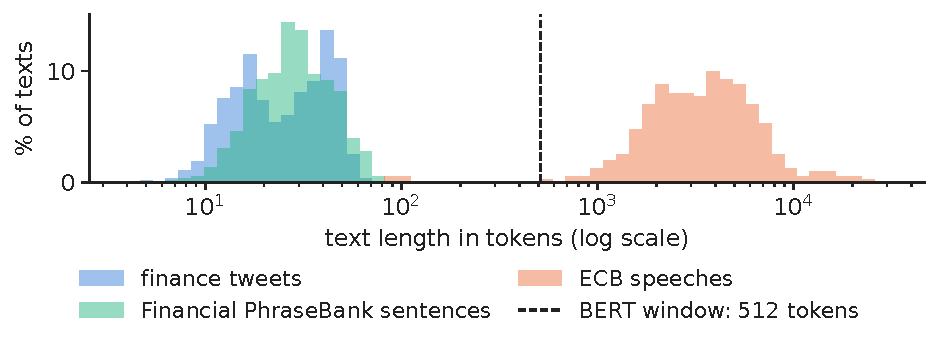
\includegraphics[width=\textwidth,height=0.383\textheight,keepaspectratio]{charts/en/context_lengths.pdf}\end{center}\vspace{-3mm}
\chartsource{Source: Twitter financial news (zeroshot); Malo et al. (2014); European Central Bank speeches; tokenizer of the ProsusAI model. Data: finance tweets; Financial PhraseBank; European Central Bank speeches 8 Jan 2022 to 30 Oct 2026.}
\vspace{0.5mm}
\begin{itemize}\setlength{\itemsep}{0pt}
  \item \textbf{Median length in tokens}: tweets 25, Financial PhraseBank sentences 28, European Central Bank (ECB) speeches 3\,338.
  \item \textbf{Context limit}: 98.8\,\% of the 400 speeches exceed 512 tokens
    \begin{itemize}\setlength{\itemsep}{0pt}
      \item Only 0.19\,\% of the tweets exceed 64.
    \end{itemize}
\end{itemize}
\par\vfill\manager{match the model to the text length: a tweet fits any transformer, a speech needs chunking or a long-context model.}\par\vspace{0.5mm}
\par\vfill\noindent{\scriptsize\color{FooterGray}}\hfill\qlink{NN\_L7\_context\_lengths}{Quantlets/L7/NN_L7_context_lengths}\par\vspace{0.5mm}
\end{frame}


\section{The attention mechanism}

\begin{frame}{Attention is a soft dictionary lookup}
\footnotesize
\intuition{Each word asks a question (query), every word offers a label (key) and a content (value); the answer is the values weighted by how well keys match the query.}
\begin{columns}[T,onlytextwidth]
\begin{column}{0.58\textwidth}
\[ \vy_i=\sum_{j=1}^{n}a_{ij}\,\mathbf v_j,\qquad a_{ij}=\frac{\exp\big(\mathbf q_i^{\top}\mathbf k_j/\sqrt{d_k}\big)}{\sum_{l=1}^{n}\exp\big(\mathbf q_i^{\top}\mathbf k_l/\sqrt{d_k}\big)} \]\[ \mathbf q_i=W_Q^{\top}\vx_i,\quad \mathbf k_j=W_K^{\top}\vx_j,\quad \mathbf v_j=W_V^{\top}\vx_j \]{\footnotesize\begin{itemize}\setlength{\itemsep}{0pt}
  \item \textbf{\txtwhere}
    \begin{itemize}\setlength{\itemsep}{0pt}
      \item $\vx_i\in\R^{d}$ = token representation
      \item $W_Q,W_K\in\R^{d\times d_k}$, $W_V\in\R^{d\times d_v}$ = learned projections
      \item $a_{ij}\ge0$, $\sum_j a_{ij}=1$: a probability over the words.
    \end{itemize}
\end{itemize}\par}
\end{column}
\begin{column}{0.39\textwidth}
\begin{itemize}\setlength{\itemsep}{3pt}
  \item \textbf{Hard lookup}
    \begin{itemize}\setlength{\itemsep}{0pt}
      \item A dictionary returns the value of the one matching key
    \end{itemize}
  \item \textbf{Soft lookup}
    \begin{itemize}\setlength{\itemsep}{0pt}
      \item Attention returns a blend of all values: differentiable, so $W_Q,W_K,W_V$ are learned
      \item One step between any two words, whatever their distance
    \end{itemize}
\end{itemize}
\end{column}
\end{columns}
\par\vfill\manager{each output word is a context-aware mixture: ``guidance'' can borrow meaning from ``raised'' ten words later.}\par\vspace{0.5mm}
\par\vfill\noindent{\scriptsize\color{FooterGray}(Vaswani et al., 2017; Bishop \& Bishop, 2024, sec.\ 12.1)}\hfill\tryit{notebook \S2}\par\vspace{0.5mm}
\end{frame}

\begin{frame}{In matrix form: one multiplication attends all words at once}
\footnotesize
\intuition{Stacking queries, keys and values as matrices turns attention into two matrix products and a row-wise softmax.}
\begin{columns}[T,onlytextwidth]
\begin{column}{0.58\textwidth}
\[ \operatorname{Attention}(Q,K,V)=\softmax\Big(\frac{QK^{\top}}{\sqrt{d_k}}+\mathbf M\Big)V \]\[ Q=XW_Q,\quad K=XW_K,\quad V=XW_V \]{\footnotesize\begin{itemize}\setlength{\itemsep}{0pt}
  \item \textbf{\txtwhere}
    \begin{itemize}\setlength{\itemsep}{0pt}
      \item $X\in\R^{n\times d}$ = the $n$ token representations
      \item $QK^{\top}\in\R^{n\times n}$ = all pairwise scores
      \item $\mathbf M$ = mask, $0$ for allowed pairs and $-\infty$ for padding (or for future tokens in a decoder).
    \end{itemize}
\end{itemize}\par}
\end{column}
\begin{column}{0.39\textwidth}
\begin{itemize}\setlength{\itemsep}{3pt}
  \item \textbf{Cost per layer}
    \begin{itemize}\setlength{\itemsep}{0pt}
      \item $O(n^2d)$ operations and $O(n^2)$ memory
      \item A median speech costs about 17\,828 times a median tweet
    \end{itemize}
  \item \textbf{Parallel}
    \begin{itemize}\setlength{\itemsep}{0pt}
      \item No loop over positions: graphics processors multiply the whole sentence at once
    \end{itemize}
\end{itemize}
\end{column}
\end{columns}
\par\vfill\manager{the $n^2$ term is why context windows are limited and long reports must be cut into pieces.}\par\vspace{0.5mm}
\par\vfill\noindent{\scriptsize\color{FooterGray}(Vaswani et al., 2017)}\hfill\tryit{notebook \S2}\par\vspace{0.5mm}
\end{frame}

\begin{frame}{Why divide by $\sqrt{d_k}$: keep the softmax out of saturation}
\footnotesize
\intuition{Dot products of long random vectors grow with their length; without scaling the softmax becomes one-hot and its gradient vanishes.}
\begin{columns}[T,onlytextwidth]
\begin{column}{0.58\textwidth}
\[ q_l,k_l\iid(0,1)\ \Rightarrow\ \E[\mathbf q^{\top}\mathbf k]=0,\quad \Var(\mathbf q^{\top}\mathbf k)=\sum_{l=1}^{d_k}\Var(q_lk_l)=d_k \]\[ \Var\big(\mathbf q^{\top}\mathbf k/\sqrt{d_k}\big)=1\quad\text{for every}\ d_k \]{\footnotesize\begin{itemize}\setlength{\itemsep}{0pt}
  \item \textbf{\txtwhere}
    \begin{itemize}\setlength{\itemsep}{0pt}
      \item $d_k$ = dimension of queries and keys (64 per head in BERT)
      \item With unit-variance scores the softmax spreads its mass and its Jacobian $\operatorname{diag}(\mathbf a)-\mathbf a\mathbf a^{\top}$ stays away from zero.
    \end{itemize}
\end{itemize}\par}
\end{column}
\begin{column}{0.39\textwidth}
\begin{itemize}\setlength{\itemsep}{3pt}
  \item \textbf{Without scaling}
    \begin{itemize}\setlength{\itemsep}{0pt}
      \item With $d_k=64$ the scores have standard deviation 8, so one word takes almost all the weight
    \end{itemize}
  \item \textbf{Temperature view}
    \begin{itemize}\setlength{\itemsep}{0pt}
      \item $\sqrt{d_k}$ is a fixed temperature that keeps attention soft at initialisation
    \end{itemize}
\end{itemize}
\end{column}
\end{columns}
\par\vfill\manager{a design constant, not a tuning knob: it is what lets deep stacks of attention train at all.}\par\vspace{0.5mm}
\par\vfill\noindent{\scriptsize\color{FooterGray}(Vaswani et al., 2017)}\par\vspace{0.5mm}
\end{frame}

\begin{frame}{Several heads look for several relations at once}
\footnotesize
\intuition{One head averages one kind of relation; several heads with smaller projections capture syntax, negation and entities in parallel.}
\begin{columns}[T,onlytextwidth]
\begin{column}{0.58\textwidth}
\[ \operatorname{MHA}(X)=\big[\mathbf H_1\,\|\,\cdots\,\|\,\mathbf H_h\big]W_O \]\[ \mathbf H_m=\operatorname{Attention}(XW_Q^{m},XW_K^{m},XW_V^{m}) \]{\footnotesize\begin{itemize}\setlength{\itemsep}{0pt}
  \item \textbf{\txtwhere}
    \begin{itemize}\setlength{\itemsep}{0pt}
      \item $h$ = number of heads
      \item $W_Q^m,W_K^m,W_V^m\in\R^{d\times d/h}$
      \item $\|$ = concatenation
      \item $W_O\in\R^{d\times d}$
      \item Parameters: $4d^2$ (+ biases), the same as one big head.
    \end{itemize}
\end{itemize}\par}
\end{column}
\begin{column}{0.39\textwidth}
\begin{itemize}\setlength{\itemsep}{3pt}
  \item \textbf{BERT-base}
    \begin{itemize}\setlength{\itemsep}{0pt}
      \item 12 layers $\times$ 12 heads, $d=$ 768, $d/h=$ 64
    \end{itemize}
  \item \textbf{Our small transformer}
    \begin{itemize}\setlength{\itemsep}{0pt}
      \item 2 layers $\times$ 4 heads, $d=64$, $d/h=16$
    \end{itemize}
\end{itemize}
\end{column}
\end{columns}
\par\vfill\manager{heads are cheap specialists: same cost as one head, more kinds of context per layer.}\par\vspace{0.5mm}
\par\vfill\noindent{\scriptsize\color{FooterGray}(Vaswani et al., 2017; Clark et al., 2019)}\hfill\tryit{notebook \S2}\par\vspace{0.5mm}
\end{frame}

\begin{frame}{What FinBERT attends to in a real bearish tweet}
\small
\begin{center}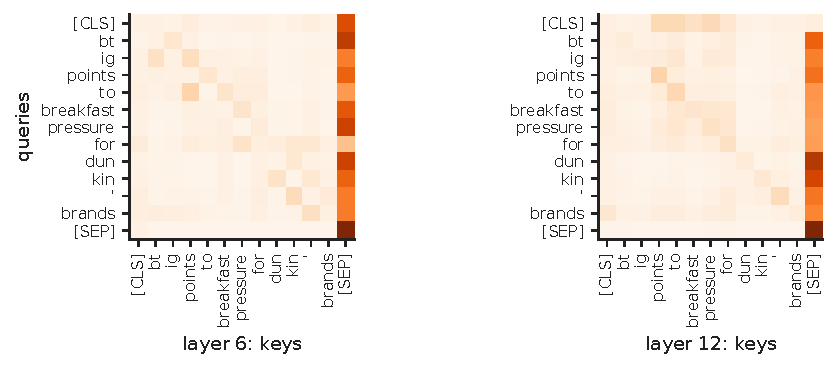
\includegraphics[width=\textwidth,height=0.523\textheight,keepaspectratio]{charts/en/attention_example.pdf}\end{center}\vspace{-3mm}
\chartsource{Source: Twitter financial news datasets (Hugging Face, zeroshot). Data: one test tweet; pretrained FinBERT, attention averaged over 12 heads.}
\vspace{0.5mm}
\begin{itemize}\setlength{\itemsep}{0pt}
  \item \textbf{Tweet} (test set, label bearish): ``BTIG points to breakfast pressure for Dunkin' Brands''
    \begin{itemize}\setlength{\itemsep}{0pt}
      \item Pretrained FinBERT gives it only 7.3\,\% probability of negative: the bearish tone is implicit.
    \end{itemize}
  \item \textbf{Layer 6}: the [CLS] token puts 5.7\,\% of its attention on ``points''
    \begin{itemize}\setlength{\itemsep}{0pt}
      \item In layer 12 most weight flows to the separator tokens.
    \end{itemize}
\end{itemize}
\par\vfill\noindent{\scriptsize\color{FooterGray}(own computation; mean over the 12 heads)}\hfill\qlink{NN\_L7\_attention\_example}{Quantlets/L7/NN_L7_attention_example}\par\vspace{0.5mm}
\end{frame}

\begin{frame}{Across layers, attention becomes concentrated on separator tokens}
\small
\begin{center}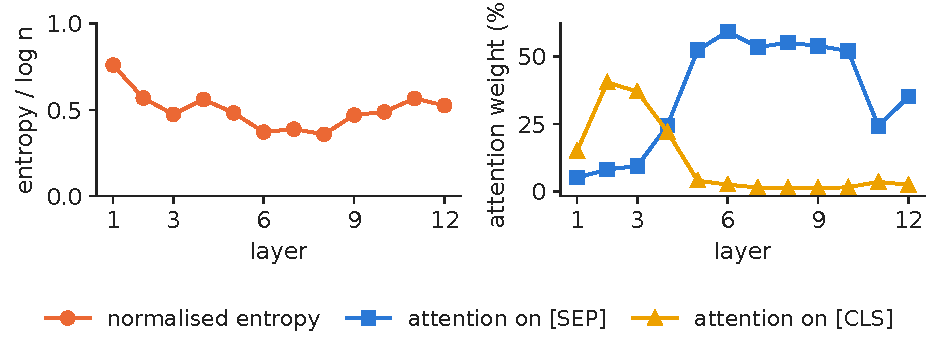
\includegraphics[width=\textwidth,height=0.520\textheight,keepaspectratio]{charts/en/attention_entropy.pdf}\end{center}\vspace{-3mm}
\chartsource{Source: Twitter financial news datasets (Hugging Face, zeroshot). Data: 500 test tweets; pretrained FinBERT.}
\vspace{0.5mm}
\begin{itemize}\setlength{\itemsep}{0pt}
  \item \textbf{Entropy} of the attention rows, divided by $\log n$: 0.76 in layer 1, lowest 0.36 in layer 8 (1 = uniform).
  \item \textbf{[SEP] as a sink}: up to 59.3\,\% of all attention (layer 6) goes to the separator: a ``no-op'' a head uses when it has nothing to add.
\end{itemize}
\par\vfill\noindent{\scriptsize\color{FooterGray}(own computation, 500 test tweets; Clark et al., 2019)}\hfill\qlink{NN\_L7\_attention\_entropy}{Quantlets/L7/NN_L7_attention_entropy}\par\vspace{0.5mm}
\end{frame}

\begin{frame}{Attention weights as explanations: limitations}
\footnotesize
\intuition{Where a head looks is not the same as why the model decides: values, later layers and the classifier all transform what attention selects.}
\begin{columns}[T,onlytextwidth]
\begin{column}{0.58\textwidth}
\[ \vh_i^{(l+1)}=\vh_i^{(l)}+\sum_{m=1}^{h}\sum_{j}a_{ij}^{(l,m)}\,W_O^{m\top}W_V^{m\top}\vh_j^{(l)}+\dots \]{\footnotesize\begin{itemize}\setlength{\itemsep}{0pt}
  \item \textbf{\txtwhere}
    \begin{itemize}\setlength{\itemsep}{0pt}
      \item The contribution of word $j$ is $a_{ij}$ times a value vector whose norm can be large or small
      \item The residual stream $\vh_i^{(l)}$ carries information that attention never touches.
    \end{itemize}
\end{itemize}\par}
\end{column}
\begin{column}{0.39\textwidth}
\begin{itemize}\setlength{\itemsep}{3pt}
  \item \textbf{Evidence}
    \begin{itemize}\setlength{\itemsep}{0pt}
      \item Different attention maps can give the same prediction (Jain \& Wallace, 2019)
      \item Heavy attention on [SEP] carries almost no information (Clark et al., 2019)
    \end{itemize}
  \item \textbf{Better tools}
    \begin{itemize}\setlength{\itemsep}{0pt}
      \item Gradient-based attributions and occlusion tests (Lecture 11)
    \end{itemize}
\end{itemize}
\end{column}
\end{columns}
\par\vfill\manager{never show an attention map to a regulator as ``the reason'' for a decision.}\par\vspace{0.5mm}
\par\vfill\noindent{\scriptsize\color{FooterGray}(Jain \& Wallace, 2019; Clark et al., 2019)}\par\vspace{0.5mm}
\end{frame}


\section{The transformer architecture}

\begin{frame}{Sinusoidal positional encoding}
\small
\begin{center}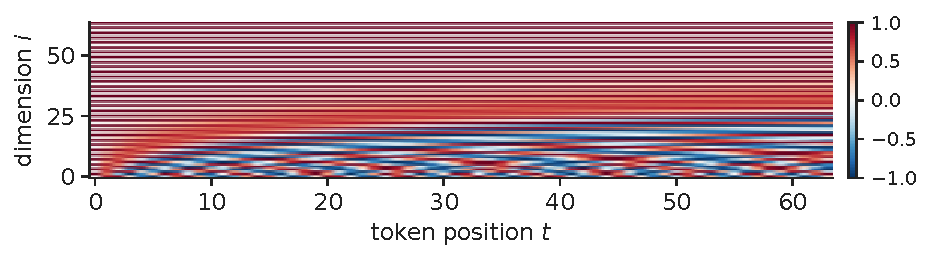
\includegraphics[width=\textwidth,height=0.480\textheight,keepaspectratio]{charts/en/positional_encoding.pdf}\end{center}\vspace{-3mm}
\chartsource{Source: Vaswani et al. (2017), sinusoidal formula. Data: mechanism illustration, $d=64$, 64 positions.}
\vspace{0.5mm}
\begin{itemize}\setlength{\itemsep}{0pt}
  \item \textbf{Formula}: $p_{t,2i}=\sin(t/10000^{2i/d})$, $p_{t,2i+1}=\cos(t/10000^{2i/d})$, added to the token embedding
    \begin{itemize}\setlength{\itemsep}{0pt}
      \item Low dimensions change fast, high ones slowly.
    \end{itemize}
  \item \textbf{Why}: self-attention is permutation-equivariant
    \begin{itemize}\setlength{\itemsep}{0pt}
      \item Without positions ``rates cut, stocks up'' equals ``stocks cut, rates up''.
    \end{itemize}
\end{itemize}
\par\vfill\noindent{\scriptsize\color{FooterGray}\simlabel\ (Vaswani et al., 2017)}\hfill\qlink{NN\_L7\_positional\_encoding}{Quantlets/L7/NN_L7_positional_encoding}\par\vspace{0.5mm}
\end{frame}

\begin{frame}{A transformer block: attention, feed-forward, residuals, normalisation}
\footnotesize
\intuition{Attention mixes information across words; a small two-layer network then transforms each word on its own; residual links and layer normalisation keep training stable.}
\begin{columns}[T,onlytextwidth]
\begin{column}{0.58\textwidth}
\[ Z=X+\operatorname{MHA}\big(\operatorname{LN}(X)\big),\qquad X'=Z+\operatorname{FFN}\big(\operatorname{LN}(Z)\big) \]\[ \operatorname{FFN}(\vz)=W_2\,\operatorname{GELU}(W_1\vz+\vb_1)+\vb_2,\quad \operatorname{LN}(\vz)=\boldsymbol\gamma\odot\frac{\vz-\mu_{\vz}}{\sigma_{\vz}}+\boldsymbol\beta \]{\footnotesize\begin{itemize}\setlength{\itemsep}{0pt}
  \item \textbf{\txtwhere}
    \begin{itemize}\setlength{\itemsep}{0pt}
      \item Pre-norm variant
      \item Position-wise feed-forward network (FFN), $W_1\in\R^{4d\times d}$
      \item Gaussian error linear unit (GELU) or rectified linear unit (ReLU)
      \item Layer normalisation (LN) over the $d$ features of one token
      \item Parameters per block $\approx12d^2$.
    \end{itemize}
\end{itemize}\par}
\end{column}
\begin{column}{0.39\textwidth}
\begin{itemize}\setlength{\itemsep}{3pt}
  \item \textbf{Residuals}
    \begin{itemize}\setlength{\itemsep}{0pt}
      \item Gradients reach early layers directly (Lecture 4)
    \end{itemize}
  \item \textbf{Our block}
    \begin{itemize}\setlength{\itemsep}{0pt}
      \item $d=64$, FFN width 128, dropout 0.1; 2 blocks: 67\,139 parameters outside the embeddings
    \end{itemize}
\end{itemize}
\end{column}
\end{columns}
\par\vfill\manager{most parameters of a transformer sit in the feed-forward layers, not in attention.}\par\vspace{0.5mm}
\par\vfill\noindent{\scriptsize\color{FooterGray}(Vaswani et al., 2017; Ba, Kiros \& Hinton, 2016)}\hfill\tryit{notebook \S3}\par\vspace{0.5mm}
\end{frame}

\begin{frame}{Encoders and decoders: two pretraining objectives}
\footnotesize
\intuition{The same block reads or writes, depending on the mask and the pretraining task.}
\begin{columns}[T,onlytextwidth]
\begin{column}{0.58\textwidth}
\[ \loss_{\text{MLM}}=-\sum_{i\in\mathcal M}\log p_{\btheta}\big(x_i\mid x_{\setminus\mathcal M}\big) \]\[ \loss_{\text{LM}}=-\sum_{t=1}^{n}\log p_{\btheta}\big(x_t\mid x_{<t}\big) \]{\footnotesize\begin{itemize}\setlength{\itemsep}{0pt}
  \item \textbf{\txtwhere}
    \begin{itemize}\setlength{\itemsep}{0pt}
      \item $\mathcal M$ = 15\,\% of positions, masked at random: masked language modelling (MLM)
      \item Second line: next-token prediction, causal mask $M_{ij}=-\infty$ for $j>i$.
    \end{itemize}
\end{itemize}\par}
\end{column}
\begin{column}{0.39\textwidth}
\begin{itemize}\setlength{\itemsep}{3pt}
  \item \textbf{Encoder-only}
    \begin{itemize}\setlength{\itemsep}{0pt}
      \item Bidirectional Encoder Representations from Transformers (BERT): classification, extraction
    \end{itemize}
  \item \textbf{Decoder-only}
    \begin{itemize}\setlength{\itemsep}{0pt}
      \item Generative Pre-trained Transformer (GPT): text generation, today's large language models (LLM)
    \end{itemize}
\end{itemize}
\end{column}
\end{columns}
\par\vfill\manager{for labelling texts use an encoder
    \begin{itemize}\setlength{\itemsep}{0pt}
      \item For writing reports use a decoder (Lecture 12).
    \end{itemize}}\par\vspace{0.5mm}
\par\vfill\noindent{\scriptsize\color{FooterGray}(Devlin et al., 2019; Radford et al., 2018)}\par\vspace{0.5mm}
\end{frame}

\begin{frame}{Text becomes numbers through subword tokens}
\footnotesize
\intuition{A fixed vocabulary of word pieces covers any word, including tickers and new company names, by splitting rare words into frequent pieces.}
\begin{columns}[T,onlytextwidth]
\begin{column}{0.58\textwidth}
\[ x_{1:n}=\big[\texttt{[CLS]},w_1,\dots,w_{n-2},\texttt{[SEP]}\big],\qquad \vx_t=E[x_t]+\mathbf p_t+\mathbf s_t \]{\footnotesize\begin{itemize}\setlength{\itemsep}{0pt}
  \item \textbf{\txtwhere}
    \begin{itemize}\setlength{\itemsep}{0pt}
      \item $E\in\R^{|\mathcal V|\times d}$ = embedding table
      \item $\mathbf p_t$ = position, $\mathbf s_t$ = segment embedding
      \item [CLS] summarises the text, [SEP] closes it
      \item WordPiece vocabulary of FinBERT: $|\mathcal V|=$ 30\,522.
    \end{itemize}
\end{itemize}\par}
\end{column}
\begin{column}{0.39\textwidth}
\begin{itemize}\setlength{\itemsep}{3pt}
  \item \textbf{Our tweets}
    \begin{itemize}\setlength{\itemsep}{0pt}
      \item Median 25 tokens, 99th percentile 57, maximum 82
      \item We cut at 64 tokens: 0.19\,\% of the tweets lose a few tokens
    \end{itemize}
  \item \textbf{Embeddings dominate small models}
    \begin{itemize}\setlength{\itemsep}{0pt}
      \item Small transformer: 2\,020\,547 parameters, of which 67\,139 outside the table
    \end{itemize}
\end{itemize}
\end{column}
\end{columns}
\par\vfill\manager{check how a tokenizer splits your tickers and product names before trusting a model on them.}\par\vspace{0.5mm}
\par\vfill\noindent{\scriptsize\color{FooterGray}(Wu et al., 2016; Devlin et al., 2019)}\hfill\tryit{notebook \S1}\par\vspace{0.5mm}
\end{frame}

\begin{frame}{Attention, recurrence and convolution compared}
\footnotesize
{\footnotesize\renewcommand{\arraystretch}{1.3}\setlength{\tabcolsep}{4pt}
\begin{tabular}{@{}p{0.26\textwidth}p{0.20\textwidth}p{0.22\textwidth}p{0.22\textwidth}@{}}\toprule
Layer type & Cost per layer & Sequential steps & Longest path \\ \midrule
Self-attention & $O(n^2 d)$ & $O(1)$ & $O(1)$ \\
Recurrent (RNN, LSTM) & $O(n d^2)$ & $O(n)$ & $O(n)$ \\
Convolution, kernel $k$ & $O(k n d^2)$ & $O(1)$ & $O(\log_k n)$ \\
\bottomrule\end{tabular}}
\vspace{2mm}
\begin{itemize}\setlength{\itemsep}{2pt}
  \item \textbf{Recurrent neural network (RNN)}: cheap per step, slow per sentence, long paths
    \begin{itemize}\setlength{\itemsep}{0pt}
      \item \textbf{convolutional neural network (CNN)}: parallel, but needs depth to link distant words.
    \end{itemize}
  \item \textbf{Self-attention}: constant path and full parallelism, paid with $n^2$ memory
    \begin{itemize}\setlength{\itemsep}{0pt}
      \item For tweets ($n\approx$ 25) the quadratic term is negligible.
    \end{itemize}
\end{itemize}
\par\vfill\noindent{\scriptsize\color{FooterGray}(Vaswani et al., 2017, Table 1)}\par\vspace{0.5mm}
\end{frame}


\section{Case study: sentiment of finance tweets}

\begin{frame}{Seven models evaluated on a common test set}
\footnotesize
{\scriptsize\renewcommand{\arraystretch}{1.05}\setlength{\tabcolsep}{4pt}
\begin{tabular}{@{}p{0.30\textwidth}p{0.62\textwidth}@{}}\toprule
Model & What is trained \\ \midrule
TF-IDF + logistic & logistic regression on word 1--2-grams (17\,119 features), $C$ chosen on validation \\
Embedding bag & mean of learned token embeddings, no attention \\
Small transformer & 2 blocks, 4 heads, $d=64$, from scratch; also without positions \\
FinBERT zero-shot & BERT further trained on financial text (FinBERT, Araci, 2019), used as is \\
FinBERT frozen + logistic & logistic regression on the mean last-layer vector (768) \\
FinBERT fine-tuned & all 109.5 million weights, 3 epochs \\
\bottomrule\end{tabular}}
\vspace{1mm}
\begin{itemize}\setlength{\itemsep}{2pt}
  \item \textbf{Split}: published training tweets = 8\,588 training + 955 validation (10\,\%, stratified)
    \begin{itemize}\setlength{\itemsep}{0pt}
      \item The published validation set = our test (2\,388), used once.
    \end{itemize}
  \item \textbf{Why not Financial PhraseBank}: FinBERT was fine-tuned on it, so testing there would leak
    \begin{itemize}\setlength{\itemsep}{0pt}
      \item Tweets are new to every model.
    \end{itemize}
\end{itemize}
\par\vfill\noindent{\scriptsize\color{FooterGray}(Araci, 2019; Malo et al., 2014)}\hfill\tryit{notebook \S5}\par\vspace{0.5mm}
\end{frame}

\begin{frame}{Our small transformer, trained from scratch}
\footnotesize
\intuition{Two blocks on top of token and position embeddings, mean-pooled over the real tokens, then a linear layer to the three classes.}
\begin{columns}[T,onlytextwidth]
\begin{column}{0.58\textwidth}
\[ \vh=\frac{1}{n}\sum_{t=1}^{n}\vx_t^{(2)},\qquad \loss=-\frac1N\sum_{i=1}^{N}w_{y_i}\log\softmax(W\vh_i+\vb)_{y_i} \]{\footnotesize\begin{itemize}\setlength{\itemsep}{0pt}
  \item \textbf{\txtwhere}
    \begin{itemize}\setlength{\itemsep}{0pt}
      \item $\vx_t^{(2)}$ = output of the second block for token $t$
      \item $w_c$ = class weight, inversely proportional to the class frequency
      \item Adam with decoupled weight decay (AdamW), learning rate $5\cdot10^{-4}$, batch 64, early stopping on validation macro-F1.
    \end{itemize}
\end{itemize}\par}
\end{column}
\begin{column}{0.39\textwidth}
\begin{itemize}\setlength{\itemsep}{3pt}
  \item \textbf{Size}
    \begin{itemize}\setlength{\itemsep}{0pt}
      \item 2\,020\,547 parameters, mostly the embedding table
    \end{itemize}
  \item \textbf{Cost}
    \begin{itemize}\setlength{\itemsep}{0pt}
      \item 44 s per seed; median 20 epochs before stopping
    \end{itemize}
  \item \textbf{Macro-F1}
    \begin{itemize}\setlength{\itemsep}{0pt}
      \item Mean of the three per-class F1 scores: bearish counts as much as neutral
    \end{itemize}
\end{itemize}
\end{column}
\end{columns}
\par\vfill\manager{macro-F1 is the right yardstick when the rare class (bearish news) is the one that costs money.}\par\vspace{0.5mm}
\par\vfill\noindent{\scriptsize\color{FooterGray}(Loshchilov \& Hutter, 2019)}\hfill\tryit{notebook \S5}\par\vspace{0.5mm}
\end{frame}

\begin{frame}{The small transformer overfits: the validation loss turns up after a few epochs}
\small
\begin{center}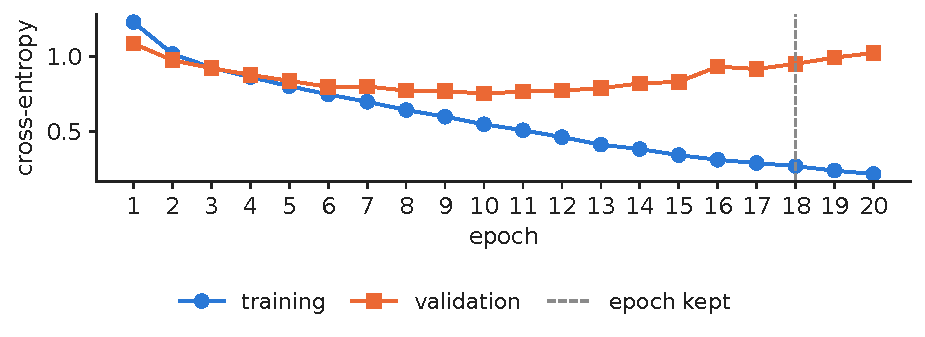
\includegraphics[width=\textwidth,height=0.500\textheight,keepaspectratio]{charts/en/tiny_learning_curve.pdf}\end{center}\vspace{-3mm}
\chartsource{Source: Twitter financial news datasets (Hugging Face, zeroshot). Data: own estimates; small transformer, seed 1.}
\vspace{0.5mm}
\begin{itemize}\setlength{\itemsep}{0pt}
  \item \textbf{Seed 1}: the validation loss is lowest at epoch 10 (0.753) and rises to 1.024 by epoch 20
    \begin{itemize}\setlength{\itemsep}{0pt}
      \item The macro-F1 used for stopping still peaks at epoch 18.
    \end{itemize}
  \item \textbf{Data-hungry}: 8\,588 tweets are few for 2\,020\,547 parameters learned from nothing
    \begin{itemize}\setlength{\itemsep}{0pt}
      \item The model grows overconfident before it stops improving.
    \end{itemize}
\end{itemize}
\par\vfill\noindent{\scriptsize\color{FooterGray}}\hfill\qlink{NN\_L7\_tiny\_learning\_curve}{Quantlets/L7/NN_L7_tiny_learning_curve}\par\vspace{0.5mm}
\end{frame}

\begin{frame}{Comparison of the models: macro-F1 on the test set}
\small
\begin{center}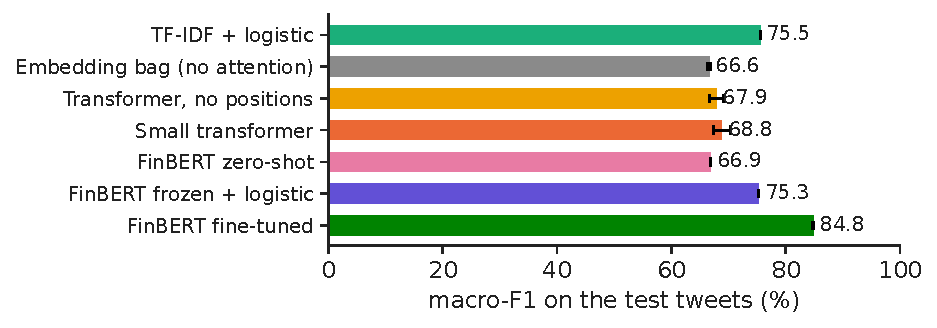
\includegraphics[width=\textwidth,height=0.542\textheight,keepaspectratio]{charts/en/model_comparison.pdf}\end{center}\vspace{-3mm}
\chartsource{Source: Twitter financial news datasets (Hugging Face, zeroshot). Data: own estimates; 2,388 test tweets (published validation split).}
\vspace{0.5mm}
\begin{itemize}\setlength{\itemsep}{0pt}
  \item \textbf{Macro-F1 on 2\,388 test tweets}: FinBERT fine-tuned 84.8\,\%, TF-IDF 75.5\,\%, small transformer 68.8\,\% (sd 1.5, 3 seeds).
  \item \textbf{FinBERT without training on tweets}: 66.9\,\%
    \begin{itemize}\setlength{\itemsep}{0pt}
      \item Frozen FinBERT + logistic: 75.3\,\%.
    \end{itemize}
\end{itemize}
\par\vfill\noindent{\scriptsize\color{FooterGray}}\hfill\qlink{NN\_L7\_model\_comparison}{Quantlets/L7/NN_L7_model_comparison}\par\vspace{0.5mm}
\end{frame}

\begin{frame}{The bearish class is where models differ most}
\footnotesize
{\scriptsize\renewcommand{\arraystretch}{1.15}\setlength{\tabcolsep}{4pt}
\begin{tabular}{@{}lrrrrr@{}}\toprule
Model & Macro-F1 & Accuracy & Bearish recall & Bearish precision & Runs \\ \midrule
TF-IDF + logistic & \cellcolor{Crimson!1}75.5 & \cellcolor{Forest!8}81.5 & \cellcolor{Crimson!5}70.3 & \cellcolor{Forest!4}63.5 & 1 \\
Embedding bag & \cellcolor{Crimson!55}66.6 & \cellcolor{Crimson!43}74.3 & \cellcolor{Crimson!44}62.0 & \cellcolor{Crimson!55}46.6 & 3 \\
Transformer, no positions & \cellcolor{Crimson!47}67.9 & \cellcolor{Crimson!35}75.4 & \cellcolor{Crimson!45}61.8 & \cellcolor{Crimson!49}48.4 & 3 \\
Small transformer & \cellcolor{Crimson!42}68.8 & \cellcolor{Crimson!26}76.7 & \cellcolor{Crimson!55}59.7 & \cellcolor{Crimson!39}51.1 & 3 \\
FinBERT zero-shot & \cellcolor{Crimson!53}66.9 & \cellcolor{Crimson!55}72.6 & \cellcolor{Forest!23}76.1 & \cellcolor{Crimson!45}49.4 & 1 \\
FinBERT frozen + logistic & \cellcolor{Crimson!2}75.3 & \cellcolor{Crimson!2}80.1 & \cellcolor{Forest!35}78.7 & \cellcolor{Crimson!13}58.6 & 1 \\
FinBERT fine-tuned & \cellcolor{Forest!55}84.8 & \cellcolor{Forest!55}88.2 & \cellcolor{Forest!55}82.9 & \cellcolor{Forest!55}77.9 & 3 \\
\bottomrule\end{tabular}}
\vspace{1.5mm}
\begin{itemize}\setlength{\itemsep}{2pt}
  \item \textbf{All numbers in \%}, test tweets
    \begin{itemize}\setlength{\itemsep}{0pt}
      \item Green = best, red = worst in the column
      \item Means over the runs.
    \end{itemize}
  \item \textbf{Bearish news}: fine-tuned FinBERT finds 82.9\,\% of them with 77.9\,\% precision
    \begin{itemize}\setlength{\itemsep}{0pt}
      \item TF-IDF 70.3\,\% and 63.5\,\%.
    \end{itemize}
\end{itemize}
\par\vfill\manager{report per-class recall and precision: an average can hide a model that misses the news that matter.}\par\vspace{0.5mm}
\par\vfill\noindent{\scriptsize\color{FooterGray}(own computation)}\hfill\tryit{notebook \S5}\par\vspace{0.5mm}
\end{frame}

\begin{frame}{Paired bootstrap test of the differences on the test tweets}
\footnotesize
\intuition{Resampling the test tweets, with the same draw for both models, shows how much a gap in macro-F1 could move by chance.}
\begin{columns}[T,onlytextwidth]
\begin{column}{0.58\textwidth}
\[ \Delta^{*b}=F_1^{A}(\mathcal T^{*b})-F_1^{B}(\mathcal T^{*b}),\quad b=1,\dots,1000 \]\[ \text{CI}_{95\%}=[q_{0.025},q_{0.975}] \]{\footnotesize\begin{itemize}\setlength{\itemsep}{0pt}
  \item \textbf{\txtwhere}
    \begin{itemize}\setlength{\itemsep}{0pt}
      \item $\mathcal T^{*b}$ = test tweets drawn with replacement
      \item $F_1$ = macro-F1 averaged over the seeds of the model
      \item Differences in percentage points.
    \end{itemize}
\end{itemize}\par}
\end{column}
\begin{column}{0.39\textwidth}
\begin{itemize}\setlength{\itemsep}{2pt}
  \item \textbf{FinBERT fine-tuned $-$ TF-IDF}
    \begin{itemize}\setlength{\itemsep}{0pt}
      \item \ensuremath{+}9.3 [\ensuremath{+}7.3; \ensuremath{+}11.3]
    \end{itemize}
  \item \textbf{Small transformer $-$ TF-IDF}
    \begin{itemize}\setlength{\itemsep}{0pt}
      \item \ensuremath{-}6.6 [\ensuremath{-}8.3; \ensuremath{-}4.9]
    \end{itemize}
  \item \textbf{With $-$ without positions}
    \begin{itemize}\setlength{\itemsep}{0pt}
      \item \ensuremath{+}0.9 [\ensuremath{+}0.1; \ensuremath{+}1.7]
    \end{itemize}
  \item \textbf{Frozen FinBERT $-$ TF-IDF}
    \begin{itemize}\setlength{\itemsep}{0pt}
      \item \ensuremath{-}0.2 [\ensuremath{-}2.5; \ensuremath{+}2.0]
    \end{itemize}
\end{itemize}
\end{column}
\end{columns}
\par\vfill\manager{an interval that excludes zero is the minimum evidence before replacing a production model.}\par\vspace{0.5mm}
\par\vfill\noindent{\scriptsize\color{FooterGray}(Efron \& Tibshirani, 1993)}\hfill\tryit{notebook \S5}\par\vspace{0.5mm}
\end{frame}

\begin{frame}{With little labelled data, pretrained representations matter most}
\small
\begin{center}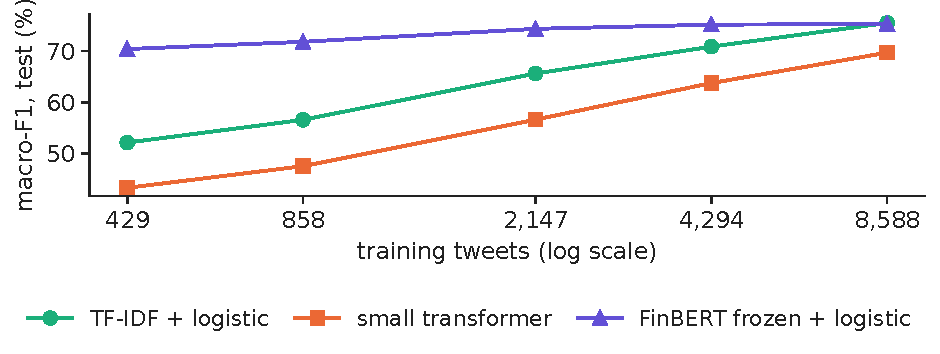
\includegraphics[width=\textwidth,height=0.520\textheight,keepaspectratio]{charts/en/data_scaling.pdf}\end{center}\vspace{-3mm}
\chartsource{Source: Twitter financial news datasets (Hugging Face, zeroshot). Data: own estimates; 2,388 test tweets (published validation split).}
\vspace{0.5mm}
\begin{itemize}\setlength{\itemsep}{0pt}
  \item \textbf{With 429 training tweets}: frozen FinBERT + logistic 70.4\,\%, TF-IDF 52.1\,\%, small transformer 43.3\,\% macro-F1.
  \item \textbf{Pretraining = data you did not label}: billions of words already shaped the FinBERT vectors
    \begin{itemize}\setlength{\itemsep}{0pt}
      \item A model from scratch must learn language and task at once.
    \end{itemize}
\end{itemize}
\par\vfill\noindent{\scriptsize\color{FooterGray}(own computation, seed 1)}\hfill\qlink{NN\_L7\_data\_scaling}{Quantlets/L7/NN_L7_data_scaling}\par\vspace{0.5mm}
\end{frame}

\begin{frame}{Fine-tuning fixes what the zero-shot model gets wrong}
\small
\begin{center}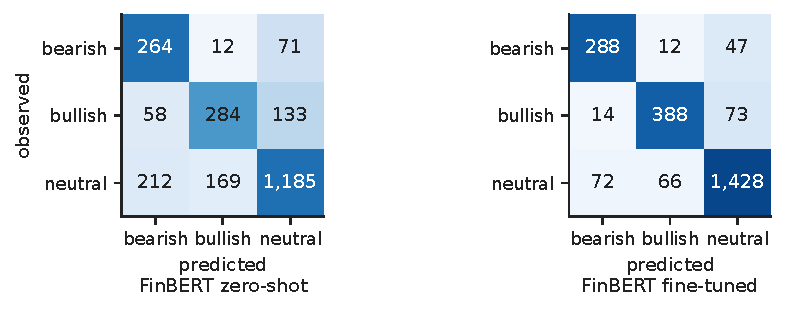
\includegraphics[width=\textwidth,height=0.520\textheight,keepaspectratio]{charts/en/confusion.pdf}\end{center}\vspace{-3mm}
\chartsource{Source: Twitter financial news datasets (Hugging Face, zeroshot). Data: own estimates; 2,388 test tweets (published validation split).}
\vspace{0.5mm}
\begin{itemize}\setlength{\itemsep}{0pt}
  \item \textbf{Zero-shot}: FinBERT was trained on news sentences, not tweets
    \begin{itemize}\setlength{\itemsep}{0pt}
      \item It finds 264 of the 347 bearish tweets
      \item After fine-tuning: 288.
    \end{itemize}
  \item \textbf{Remaining errors}: 47 bearish and 73 bullish tweets read as neutral
    \begin{itemize}\setlength{\itemsep}{0pt}
      \item Only 12 bearish read as bullish.
    \end{itemize}
\end{itemize}
\par\vfill\noindent{\scriptsize\color{FooterGray}(own computation, fine-tuned model of seed 1)}\hfill\qlink{NN\_L7\_confusion}{Quantlets/L7/NN_L7_confusion}\par\vspace{0.5mm}
\end{frame}

\begin{frame}{Fine-tuning: start from pretrained weights, take small steps}
\footnotesize
\intuition{All weights move, but only a little: the language knowledge stays, the decision layer adapts to tweets.}
\begin{columns}[T,onlytextwidth]
\begin{column}{0.58\textwidth}
\[ \btheta_0=\btheta_{\text{FinBERT}},\qquad \btheta_{s+1}=\btheta_s-\eta_s\,\widehat{\nabla\loss}(\btheta_s),\quad \eta_s=\eta_0\Big(1-\frac{s}{S}\Big) \]{\footnotesize\begin{itemize}\setlength{\itemsep}{0pt}
  \item \textbf{\txtwhere}
    \begin{itemize}\setlength{\itemsep}{0pt}
      \item $\eta_0=2\cdot10^{-5}$, linear decay over $S$ = 3 epochs of batches of 32
      \item AdamW with weight decay 0.01
      \item The epoch with the best validation macro-F1 is kept.
    \end{itemize}
\end{itemize}\par}
\end{column}
\begin{column}{0.39\textwidth}
\begin{itemize}\setlength{\itemsep}{3pt}
  \item \textbf{Gain}
    \begin{itemize}\setlength{\itemsep}{0pt}
      \item \ensuremath{+}17.9 points over zero-shot, \ensuremath{+}9.3 over TF-IDF
    \end{itemize}
  \item \textbf{Cost}
    \begin{itemize}\setlength{\itemsep}{0pt}
      \item 109.5 million weights, 5.2 minutes per seed on a laptop graphics processor
    \end{itemize}
  \item \textbf{Risk}
    \begin{itemize}\setlength{\itemsep}{0pt}
      \item A large learning rate erases pretraining (catastrophic forgetting)
    \end{itemize}
\end{itemize}
\end{column}
\end{columns}
\par\vfill\manager{fine-tuning a pretrained encoder is today's default for any labelled text task with a few thousand examples.}\par\vspace{0.5mm}
\par\vfill\noindent{\scriptsize\color{FooterGray}(Devlin et al., 2019; Araci, 2019)}\hfill\tryit{notebook \S5}\par\vspace{0.5mm}
\end{frame}

\begin{frame}{Does word order matter for tweets?}
\footnotesize
\begin{columns}[T,onlytextwidth]
\begin{column}{0.49\textwidth}
\begin{itemize}\setlength{\itemsep}{5pt}
  \item \textbf{Ablation}
    \begin{itemize}\setlength{\itemsep}{0pt}
      \item Same small transformer with and without positional encoding, 3 seeds each
      \item Macro-F1 68.8\,\% with positions, 67.9\,\% without: \ensuremath{+}0.9 points
    \end{itemize}
  \item \textbf{Bootstrap}
    \begin{itemize}\setlength{\itemsep}{0pt}
      \item 95\,\% interval of the gain: [\ensuremath{+}0.1; \ensuremath{+}1.7] points
    \end{itemize}
\end{itemize}
\end{column}
\begin{column}{0.48\textwidth}
\begin{itemize}\setlength{\itemsep}{5pt}
  \item \textbf{Reading}
    \begin{itemize}\setlength{\itemsep}{0pt}
      \item Short, formulaic tweets are mostly bags of signal words (``cut'', ``beats'', ``downgrade'')
      \item The embedding bag, with no attention, is close: 66.6\,\%
    \end{itemize}
  \item \textbf{When order matters}
    \begin{itemize}\setlength{\itemsep}{0pt}
      \item Negation and contrast (``not'', ``but''), long documents, numbers attached to the right entity
    \end{itemize}
\end{itemize}
\end{column}
\end{columns}
\par\vfill\manager{test the simple version of your model first: on short texts much of the transformer's power is unused.}\par\vspace{0.5mm}
\par\vfill\noindent{\scriptsize\color{FooterGray}(own computation)}\hfill\tryit{notebook \S5}\par\vspace{0.5mm}
\end{frame}


\section{Transformers in practice}

\begin{frame}{From sentiment scores to a business signal}
\footnotesize
\begin{columns}[T,onlytextwidth]
\begin{column}{0.49\textwidth}
\begin{itemize}\setlength{\itemsep}{5pt}
  \item \textbf{Pipeline}
    \begin{itemize}\setlength{\itemsep}{0pt}
      \item Stream of news and posts $\to$ tokenizer $\to$ fine-tuned encoder $\to$ class probabilities
      \item Aggregate by firm and day: share of bearish minus bullish, weighted by reach
    \end{itemize}
  \item \textbf{Uses}
    \begin{itemize}\setlength{\itemsep}{0pt}
      \item Risk monitoring of a credit portfolio, early warning for issuers, an input to Value-at-Risk (VaR) overlays
    \end{itemize}
\end{itemize}
\end{column}
\begin{column}{0.48\textwidth}
\begin{itemize}\setlength{\itemsep}{5pt}
  \item \textbf{Pitfalls}
    \begin{itemize}\setlength{\itemsep}{0pt}
      \item Look-ahead: use only texts time-stamped before the decision
      \item Domain shift: a model of news sentences misreads tweets (zero-shot gap)
      \item Label noise and sarcasm; drift when the market vocabulary changes
    \end{itemize}
\end{itemize}
\end{column}
\end{columns}
\par\vfill\manager{a sentiment score is an input to a model, not a trading decision: backtest it before use.}\par\vspace{0.5mm}
\par\vfill\noindent{\scriptsize\color{FooterGray}(Tetlock, 2007)}\par\vspace{0.5mm}
\end{frame}

\begin{frame}{Long documents: central-bank speeches and annual reports}
\footnotesize
\begin{columns}[T,onlytextwidth]
\begin{column}{0.49\textwidth}
\begin{itemize}\setlength{\itemsep}{5pt}
  \item \textbf{Our speeches}
    \begin{itemize}\setlength{\itemsep}{0pt}
      \item 400 speeches of the ECB, 8 Jan 2022 to 30 Oct 2026
      \item Median 3\,338 tokens, longest 22\,646
    \end{itemize}
  \item \textbf{Quadratic cost}
    \begin{itemize}\setlength{\itemsep}{0pt}
      \item Attention on a median speech costs about 17\,828 times that on a median tweet
    \end{itemize}
\end{itemize}
\end{column}
\begin{column}{0.48\textwidth}
\begin{itemize}\setlength{\itemsep}{5pt}
  \item \textbf{Options}
    \begin{itemize}\setlength{\itemsep}{0pt}
      \item Chunk into windows of 512 and pool the chunk scores
      \item Hierarchical models: sentence vectors, then attention over sentences
      \item Long-context models: sparse or memory-efficient attention
    \end{itemize}
\end{itemize}
\end{column}
\end{columns}
\par\vfill\manager{for a monetary-policy desk, chunking plus a well-tested encoder usually beats an untested long-context model.}\par\vspace{0.5mm}
\par\vfill\noindent{\scriptsize\color{FooterGray}(Vaswani et al., 2017)}\hfill\tryit{notebook \S1}\par\vspace{0.5mm}
\end{frame}

\begin{frame}{Transformers beyond text}
\footnotesize
\begin{columns}[T,onlytextwidth]
\begin{column}{0.49\textwidth}
\begin{itemize}\setlength{\itemsep}{5pt}
  \item \textbf{Time series}
    \begin{itemize}\setlength{\itemsep}{0pt}
      \item Patches of a series as tokens; pretrained forecasting models (Lecture 13)
    \end{itemize}
  \item \textbf{Tables and transactions}
    \begin{itemize}\setlength{\itemsep}{0pt}
      \item Each column or each past payment as a token; attention across them
    \end{itemize}
\end{itemize}
\end{column}
\begin{column}{0.48\textwidth}
\begin{itemize}\setlength{\itemsep}{5pt}
  \item \textbf{Graphs}
    \begin{itemize}\setlength{\itemsep}{0pt}
      \item Attention restricted to the edges = graph attention network (Lecture 9)
    \end{itemize}
  \item \textbf{Images and documents}
    \begin{itemize}\setlength{\itemsep}{0pt}
      \item Image patches as tokens; vision-language models read charts and reports (Lecture 14)
    \end{itemize}
\end{itemize}
\end{column}
\end{columns}
\par\vfill\manager{whatever the data, the question is the same: what are the tokens, and which pairs may attend to each other?}\par\vspace{0.5mm}
\par\vfill\noindent{\scriptsize\color{FooterGray}(Bishop \& Bishop, 2024, ch.\ 12)}\par\vspace{0.5mm}
\end{frame}


\section{Wrap-up}

\begin{frame}{What to remember}
\small
\begin{itemize}\setlength{\itemsep}{6pt}
  \item \textbf{Attention} = softmax of scaled query-key scores times values
    \begin{itemize}\setlength{\itemsep}{0pt}
      \item One step between any two words, $O(n^2)$ cost
      \item $\sqrt{d_k}$ keeps the softmax trainable.
    \end{itemize}
  \item \textbf{Transformer block} = multi-head attention + feed-forward, each with a residual link and layer normalisation
    \begin{itemize}\setlength{\itemsep}{0pt}
      \item Positions are added, because attention ignores order.
    \end{itemize}
  \item \textbf{On finance tweets} pretraining decides: fine-tuned FinBERT 84.8\,\% macro-F1, TF-IDF 75.5\,\%, a transformer from scratch 68.8\,\%.
  \item \textbf{Attention maps} are clues, not explanations
    \begin{itemize}\setlength{\itemsep}{0pt}
      \item Check per-class errors and bootstrap intervals before trusting a model.
    \end{itemize}
\end{itemize}
\end{frame}

\begin{frame}{Research from our group: transformers as risk forecasters}
\footnotesize
\begin{itemize}\setlength{\itemsep}{5pt}
  \item \textbf{Large language models (LLM) as tail-risk forecasters} (Pele, Bolovăneanu, Lin, Ren, Ginavar, Spilak, Andrei, Toma, Lessmann \& Härdle, 2026): uses decoder transformers, prompted with return histories, to forecast Value-at-Risk and the expected shortfall (ES) --- LLM-VaR and LLM-ES --- and evaluates them with standard risk backtests.
  \item \textbf{Foundation models for tail risk} (Jheng, Tak, Găman, Mazurencu-Marinescu-Pele \& Pele, 2026): uses pretrained transformer forecasting models, without retraining and with conformal calibration, to forecast VaR and ES in Central and Eastern European markets.
  \item \textbf{Link with this lecture}: the same idea as FinBERT, a model pretrained on large data and used with little or no task-specific training, applied to risk numbers instead of words.
\end{itemize}
\vspace{1mm}{\scriptsize Findings as stated in the papers; the numbers on the other slides come from our own computations.}
\par\vfill\noindent{\scriptsize\color{FooterGray}(Bucharest University of Economic Studies; Romanian Academy, Institute for Economic Forecasting)}\par\vspace{0.5mm}
\end{frame}

\begin{frame}{Further reading and resources}
\small
\begin{columns}[T,onlytextwidth]
\begin{column}{0.52\textwidth}
\begin{itemize}\setlength{\itemsep}{4pt}
  \item \textbf{Vaswani et al.\ (2017)}, ``Attention is all you need'': the original transformer.
  \item \textbf{Bishop \& Bishop (2024)}, chapter 12: transformers, from attention to large language models.
  \item \textbf{The Illustrated Transformer} (J.\ Alammar): \href{https://jalammar.github.io/illustrated-transformer/}{jalammar.github.io}.
\end{itemize}
\end{column}
\begin{column}{0.45\textwidth}
\begin{itemize}\setlength{\itemsep}{4pt}
  \item \textbf{Hugging Face course}, fine-tuning encoders: \href{https://huggingface.co/learn/llm-course}{huggingface.co/learn}.
  \item \textbf{This course}: code, data, notebooks --- \href{https://github.com/danpele/NEURAL_BIZ}{github.com/danpele/NEURAL\_BIZ}.
  \item \textbf{Experiment yourself}: the notebook reproduces every chart and number of this lecture.
\end{itemize}
\end{column}
\end{columns}
\end{frame}

\begin{frame}{Quiz 1: scaling}
\small
\begin{itemize}
  \item Why are attention scores divided by $\sqrt{d_k}$?
\end{itemize}
\vspace{2mm}
\begin{exampleblock}{Answer}
\begin{itemize}
  \item With unit-variance entries the dot product $\mathbf q^{\top}\mathbf k$ has variance $d_k$
    \begin{itemize}\setlength{\itemsep}{0pt}
      \item Dividing by $\sqrt{d_k}$ brings it back to 1, so the softmax does not saturate and its gradient does not vanish.
    \end{itemize}
\end{itemize}
\end{exampleblock}
\end{frame}

\begin{frame}{Quiz 2: positions}
\small
\begin{itemize}
  \item What happens to a transformer without positional encoding?
\end{itemize}
\vspace{2mm}
\begin{exampleblock}{Answer}
\begin{itemize}
  \item Self-attention is permutation-equivariant, so the model sees a bag of tokens
    \begin{itemize}\setlength{\itemsep}{0pt}
      \item On our short tweets this cost only 0.9 points of macro-F1, but order matters for negation and long texts.
    \end{itemize}
\end{itemize}
\end{exampleblock}
\end{frame}

\begin{frame}{Quiz 3: pretraining}
\small
\begin{itemize}
  \item Why does a transformer trained from scratch on 8\,588 tweets lose to TF-IDF?
\end{itemize}
\vspace{2mm}
\begin{exampleblock}{Answer}
\begin{itemize}
  \item It must learn language and task from few examples with 2\,020\,547 parameters
    \begin{itemize}\setlength{\itemsep}{0pt}
      \item Pretrained FinBERT brings that knowledge and reaches 84.8\,\% after fine-tuning.
    \end{itemize}
\end{itemize}
\end{exampleblock}
\end{frame}

\begin{frame}{Quiz 4: encoder or decoder}
\small
\begin{itemize}
  \item A bank wants to label 10,000 complaints a day by topic.
    \begin{itemize}\setlength{\itemsep}{0pt}
      \item Encoder or decoder transformer?
    \end{itemize}
\end{itemize}
\vspace{2mm}
\begin{exampleblock}{Answer}
\begin{itemize}
  \item An encoder (BERT-type), fine-tuned on labelled complaints: it reads the whole text in both directions and outputs class probabilities, cheaply and consistently.
\end{itemize}
\end{exampleblock}
\end{frame}

\begin{frame}{Quiz 5: attention maps}
\small
\begin{itemize}
  \item Can an attention map justify a decision to a regulator?
\end{itemize}
\vspace{2mm}
\begin{exampleblock}{Answer}
\begin{itemize}
  \item No: different maps can give the same prediction, and much attention goes to [SEP] (up to 59.3\,\% here)
    \begin{itemize}\setlength{\itemsep}{0pt}
      \item Use attribution methods and tests instead.
    \end{itemize}
\end{itemize}
\end{exampleblock}
\end{frame}

\begin{frame}{References (1/2)}
\scriptsize
\begin{itemize}\setlength{\itemsep}{0pt}\scriptsize
\item Araci, D.\ (2019). FinBERT: Financial sentiment analysis with pre-trained language models. \href{https://arxiv.org/abs/1908.10063}{arXiv:1908.10063}
\item Ba, J.\,L., Kiros, J.\,R.\ \& Hinton, G.\,E.\ (2016). Layer normalization. \href{https://arxiv.org/abs/1607.06450}{arXiv:1607.06450}
\item Bahdanau, D., Cho, K.\ \& Bengio, Y.\ (2015). Neural machine translation by jointly learning to align and translate. \textit{International Conference on Learning Representations}. \href{https://arxiv.org/abs/1409.0473}{arXiv:1409.0473}
\item Bishop, C.\,M.\ \& Bishop, H.\ (2024). \textit{Deep Learning: Foundations and Concepts}, ch.\ 12. Springer. \href{https://doi.org/10.1007/978-3-031-45468-4}{doi:10.1007/978-3-031-45468-4}
\item Clark, K., Khandelwal, U., Levy, O.\ \& Manning, C.\,D.\ (2019). What does BERT look at? An analysis of BERT's attention. \textit{BlackboxNLP Workshop}, 276--286. \href{https://doi.org/10.18653/v1/W19-4828}{doi:10.18653/v1/W19-4828}
\item Devlin, J., Chang, M.-W., Lee, K.\ \& Toutanova, K.\ (2019). BERT: Pre-training of deep bidirectional transformers for language understanding. \textit{Proceedings of NAACL}, 4171--4186. \href{https://doi.org/10.18653/v1/N19-1423}{doi:10.18653/v1/N19-1423}
\item Efron, B.\ \& Tibshirani, R.\,J.\ (1993). \textit{An Introduction to the Bootstrap}. Chapman \& Hall. \href{https://doi.org/10.1201/9780429246593}{doi:10.1201/9780429246593}
\item Jain, S.\ \& Wallace, B.\,C.\ (2019). Attention is not explanation. \textit{Proceedings of NAACL}, 3543--3556. \href{https://doi.org/10.18653/v1/N19-1357}{doi:10.18653/v1/N19-1357}
\end{itemize}
\end{frame}

\begin{frame}{References (2/2)}
\scriptsize
\begin{itemize}\setlength{\itemsep}{0pt}\scriptsize
\item Jheng, S.-L., Tak, R., Găman, Ș., Mazurencu-Marinescu-Pele, M.\ \& Pele, D.\,T.\ (2026). Can foundation models manage risk? Zero-shot VaR and ES forecasting with conformal calibration in CEE markets. \textit{Economic Computation and Economic Cybernetics Studies and Research}, 60(2), 267--290. \href{https://doi.org/10.24818/18423264/60.2.26.14}{doi:10.24818/18423264/60.2.26.14}
\item Loshchilov, I.\ \& Hutter, F.\ (2019). Decoupled weight decay regularization. \textit{International Conference on Learning Representations}. \href{https://arxiv.org/abs/1711.05101}{arXiv:1711.05101}
\item Malo, P., Sinha, A., Korhonen, P., Wallenius, J.\ \& Takala, P.\ (2014). Good debt or bad debt: Detecting semantic orientations in economic texts. \textit{Journal of the Association for Information Science and Technology}, 65(4), 782--796. \href{https://doi.org/10.1002/asi.23062}{doi:10.1002/asi.23062}
\item Pele, D.\,T., Bolovăneanu, V., Lin, M.-B., Ren, R., Ginavar, A.\,T., Spilak, B., Andrei, A.-V., Toma, F.-M., Lessmann, S.\ \& Härdle, W.\,K.\ (2026). In the beginning was the word: LLM-VaR and LLM-ES. SSRN Working Paper 5104383. \href{https://doi.org/10.2139/ssrn.5104383}{doi:10.2139/ssrn.5104383}
\item Radford, A., Narasimhan, K., Salimans, T.\ \& Sutskever, I.\ (2018). Improving language understanding by generative pre-training. OpenAI technical report. \href{https://openai.com/research/language-unsupervised}{openai.com/research/language-unsupervised}
\item Tetlock, P.\,C.\ (2007). Giving content to investor sentiment: The role of media in the stock market. \textit{Journal of Finance}, 62(3), 1139--1168. \href{https://doi.org/10.1111/j.1540-6261.2007.01232.x}{doi:10.1111/j.1540-6261.2007.01232.x}
\item Vaswani, A., Shazeer, N., Parmar, N., Uszkoreit, J., Jones, L., Gomez, A.\,N., Kaiser, Ł.\ \& Polosukhin, I.\ (2017). Attention is all you need. \textit{Advances in Neural Information Processing Systems}, 30. \href{https://arxiv.org/abs/1706.03762}{arXiv:1706.03762}
\item Wu, Y., Schuster, M., Chen, Z.\ et al.\ (2016). Google's neural machine translation system: Bridging the gap between human and machine translation. \href{https://arxiv.org/abs/1609.08144}{arXiv:1609.08144}
\end{itemize}
\end{frame}

\appendix

\section*{Appendix}

\begin{frame}{Appendix A: gradient of the softmax and saturation}
\small
\begin{columns}[T,onlytextwidth]
\begin{column}{0.50\textwidth}
\[ a_j=\frac{e^{s_j}}{\sum_l e^{s_l}},\qquad \frac{\partial a_j}{\partial s_i}=a_j(\delta_{ij}-a_i) \]\[ J=\operatorname{diag}(\mathbf a)-\mathbf a\mathbf a^{\top},\qquad \|J\|\to0\ \text{when}\ \mathbf a\to\mathbf e_k \]
\end{column}
\begin{column}{0.47\textwidth}
\begin{itemize}\setlength{\itemsep}{3pt}
  \item If one score dominates, $\mathbf a$ is almost one-hot and every entry of $J$ is close to zero: the queries and keys stop learning.
  \item Scores with standard deviation $\sigma$ make domination likely when $\sigma$ is large
    \begin{itemize}\setlength{\itemsep}{0pt}
      \item Scaling by $\sqrt{d_k}$ fixes $\sigma=1$ at initialisation.
    \end{itemize}
\end{itemize}
\end{column}
\end{columns}
\par\vfill\noindent{\scriptsize\color{FooterGray}(Vaswani et al., 2017)}\par\vspace{0.5mm}
\end{frame}

\begin{frame}{Appendix B: parameters of a transformer block}
\small
\begin{columns}[T,onlytextwidth]
\begin{column}{0.50\textwidth}
\[ \underbrace{4d^2+4d}_{\text{attention}}+\underbrace{8d^2+5d}_{\text{FFN}}+\underbrace{4d}_{\text{LN}}\ \approx\ 12d^2 \]
\end{column}
\begin{column}{0.47\textwidth}
\begin{itemize}\setlength{\itemsep}{3pt}
  \item Attention: $W_Q,W_K,W_V,W_O\in\R^{d\times d}$ with biases
    \begin{itemize}\setlength{\itemsep}{0pt}
      \item FFN: $W_1\in\R^{4d\times d}$, $W_2\in\R^{d\times4d}$
      \item Two layer norms with $\boldsymbol\gamma,\boldsymbol\beta$.
    \end{itemize}
  \item BERT-base, $d=768$: about 7 million per block, 85 million in 12 blocks, plus 23 million in the embedding table (as published).
\end{itemize}
\end{column}
\end{columns}
\par\vfill\noindent{\scriptsize\color{FooterGray}(Devlin et al., 2019)}\par\vspace{0.5mm}
\end{frame}

\begin{frame}{Appendix C: settings of the experiments}
\small
{\scriptsize\renewcommand{\arraystretch}{1.05}\setlength{\tabcolsep}{4pt}
\begin{tabular}{@{}p{0.27\textwidth}p{0.66\textwidth}@{}}\toprule
Model & Settings \\ \midrule
TF-IDF & 1--2-grams, minimum 2 documents, sublinear term frequency; logistic regression with balanced class weights, $C$ = 3 chosen on validation \\
Small transformer & WordPiece tokens of FinBERT, 64 tokens; $d=64$, 4 heads, 2 pre-norm blocks, FFN 128, dropout 0.1; AdamW $5\cdot10^{-4}$, batch 64, at most 20 epochs, patience 4 \\
FinBERT fine-tuned & ProsusAI checkpoint, its own 3-class head re-mapped to bearish/bullish/neutral; AdamW $2\cdot10^{-5}$, linear decay, batch 32, 3 epochs; seeds 1--3 \\
Frozen FinBERT & mean of the last hidden layer over the real tokens; logistic regression, $C$ = 0.03 \\
Hardware & Apple-silicon laptop, graphics processor, Metal Performance Shaders (MPS); total run 8.1 minutes \\
\bottomrule\end{tabular}}
\end{frame}

\end{document}
